\RequirePackage{luatex85}
\RequirePackage{shellesc}
\documentclass[titlepage]{article}
% This report uses the following packages:
\usepackage{appendix}
\usepackage{booktabs}
\usepackage{caption}
\usepackage{listings}
\usepackage{microtype}
\usepackage{pgfplots}
\usepackage{tabularx}
\usepackage{tikz}
\usepackage{xcolor}
% This report uses the following TikZ libraries:
\usetikzlibrary{calc}
\usetikzlibrary{external}
\usetikzlibrary{plotmarks}
\immediate\write18{mkdir -p tikz-externalized}
\tikzexternalize[prefix=tikz-externalized/]
\tikzset{external/system call/.add={}{; convert -density 600 -flatten "\image.pdf" "\image-600.png"}}
% This report uses the following PGFPlots libraries:
\usepgfplotslibrary{fillbetween}
% This report sets the following listings options:
% This report sets the following PGFPlots options:
\pgfplotsset{compat=1.15}
\lstdefinelanguage{json}{%
basicstyle={\normalfont\ttfamily},%
stringstyle=\color{black!90},%
numbers=left,%
numberstyle=\scriptsize,%
stepnumber=1,%
numbersep=8pt,%
showstringspaces=false,%
breaklines=true,%
backgroundcolor=\color{gray!10},%
string=[s]{"}{"},%
comment=[l]{:\ "},%
morecomment=[l]{:"},%
literate=%
  *{0}{{{\color{black!70}0}}}{1}%
  {1}{{{\color{black!70}1}}}{1}%
  {2}{{{\color{black!70}2}}}{1}%
  {3}{{{\color{black!70}3}}}{1}%
  {4}{{{\color{black!70}4}}}{1}%
  {5}{{{\color{black!70}5}}}{1}%
  {6}{{{\color{black!70}6}}}{1}%
  {7}{{{\color{black!70}7}}}{1}%
  {8}{{{\color{black!70}8}}}{1}%
  {9}{{{\color{black!70}9}}}{1}}%
\lstset{language=json}
\definecolor{pdtblack}{RGB}{0,0,0}
\definecolor{pdtblue}{RGB}{11,93,174}
\definecolor{pdtdarkblue}{RGB}{6,26,64}
\definecolor{pdtdarkgreen}{RGB}{49,92,43}
\definecolor{pdtdarkpurple}{RGB}{50,14,59}
\definecolor{pdtdarkred}{RGB}{61,19,8}
\definecolor{pdtgray}{RGB}{120,120,120}
\definecolor{pdtgreen}{RGB}{100,161,27}
\definecolor{pdtlightblue}{RGB}{59,175,236}
\definecolor{pdtlightgreen}{RGB}{149,198,35}
\definecolor{pdtlightpurple}{RGB}{197,137,232}
\definecolor{pdtlightred}{RGB}{206,62,21}
\definecolor{pdtpurple}{RGB}{106,20,125}
\definecolor{pdtred}{RGB}{145,0,33}
\definecolor{pdtwhite}{RGB}{255,255,255}
\definecolor{pdtyellow}{RGB}{232,163,26}
\title{\bfseries\LARGE Experiment \\ \texttt{2025-09-16\_12-27-08\_defaultNarrowPassage2D}}
\author{Planner Developer Tools (PDT)}
\date{\today}

\begin{document}
\maketitle
\section{Overview}\label{sec:overview}

This report was automatically generated using Planner Developer Tools (PDT). It presents the results for the \texttt{2025-09-16\_12-27-08\_defaultNarrowPassage2D} experiment, which executed 100 runs of Informed HZ,  and Informed RRT* on the \texttt{defaultNarrowPassage2D} planning context. See appendix~\ref{sec:experiment-configuration} for more information about the experiment setup.
\subsection{Results Summary}\label{sec:overview-results-summary}
{\tiny
\setlength{\tabcolsep}{0.8em}
\begin{tabularx}{\textwidth}[c]{Xcccccccccc}\toprule
Planner & \(t_\mathrm{init}^\mathrm{min}\) & \(t_\mathrm{init}^\mathrm{med}\) & \(t_\mathrm{init}^\mathrm{max}\) & \(c_\mathrm{init}^\mathrm{min}\) & \(c_\mathrm{init}^\mathrm{med}\) & \(c_\mathrm{init}^\mathrm{max}\) & \(c_\mathrm{final}^\mathrm{min}\) & \(c_\mathrm{final}^\mathrm{med}\) & \(c_\mathrm{final}^\mathrm{max}\) & Success \\[0.5em]\midrule
Informed HZ& 0.0073 & \bfseries 0.0284 & \infty & \bfseries 0.4410 & \bfseries 0.5562 & \infty & 0.4410 & 0.5174 & \infty & \bfseries 0.92 \\[0.5em]
Informed RRT*& \bfseries 0.0067 & 0.0673 & \infty & 0.4444 & 0.5568 & \infty & \bfseries 0.4286 & \bfseries 0.4968 & \infty & 0.70 \\[0.5em]
\bottomrule
\end{tabularx}
}
\begin{center}
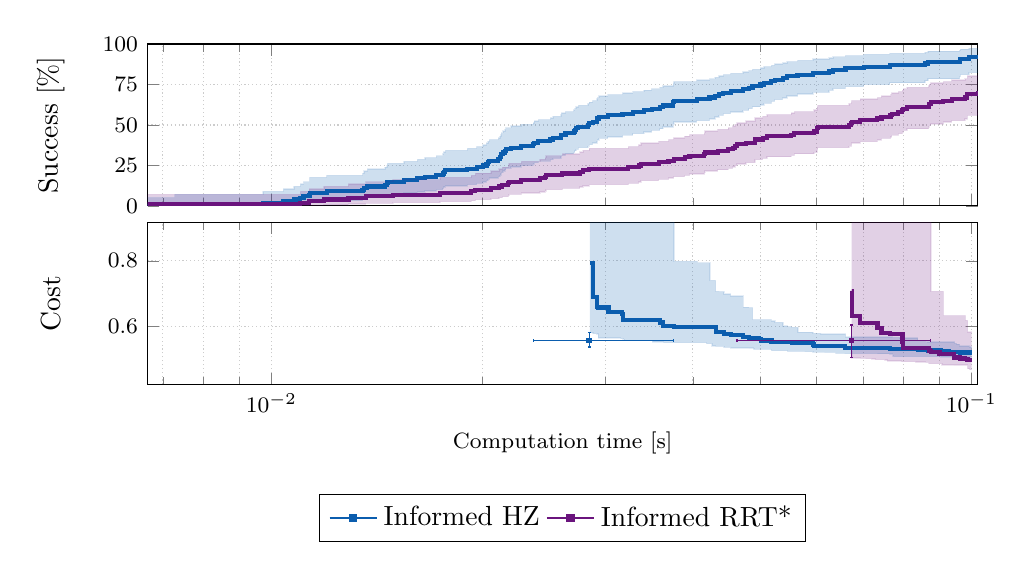
\begin{tikzpicture} [
  xscale=1,
  yscale=1
]
\begin{axis} [
  width=\textwidth,
  height=0.3\textwidth,
  at={(0cm, 0cm)},
  unbounded coords=jump,
  xtick align=inside,
  ytick align=inside,
  axis line style={solid, black},
  name=SuccessAxis,
  xmajorgrids,
  xminorgrids,
  ymajorgrids,
  major grid style={densely dotted, black!20},
  minor grid style={densely dotted, black!20},
  xmin=0.00665588,
  xmax=0.102103,
  ymin=0,
  ymax=100,
  xmode=log,
  xlabel={{\empty}},
  xlabel style={font=\footnotesize},
  xticklabel={{\empty}},
  xticklabel style={font=\footnotesize},
  ylabel={Success [\%]},
  ylabel style={font=\footnotesize, text depth=0.0em, text height=0.5em},
  ylabel absolute,
  ytick={0,25,50,75,100},
  yticklabel style={font=\footnotesize}
]
\addplot [
  line width=0.5,
  color=pdtblue,
  mark="none",
  const plot,
  name path={defaultInformedHZSuccessUpperConfidence},
  fill opacity=0.2,
  draw opacity=0.1
] table [
  row sep=\\,
  col sep=&
]{
1e-09 & 5.1604\\
0.00727877 & 7.19577\\
0.00973225 & 8.94307\\
0.0104066 & 10.5481\\
0.0107682 & 12.0633\\
0.010999 & 13.5145\\
0.0111162 & 14.9169\\
0.0113376 & 16.2803\\
0.0113403 & 17.6114\\
0.0119951 & 18.9152\\
0.013495 & 20.1954\\
0.0135649 & 21.4547\\
0.013711 & 22.6955\\
0.0145303 & 23.9196\\
0.0146348 & 25.1285\\
0.0146493 & 26.3235\\
0.0154656 & 27.5057\\
0.0161594 & 28.676\\
0.0165704 & 29.8351\\
0.0172065 & 30.9838\\
0.0175742 & 32.1226\\
0.0176248 & 33.2522\\
0.0177204 & 34.3729\\
0.0190552 & 35.4851\\
0.0196488 & 36.5893\\
0.0200467 & 37.6857\\
0.0202887 & 38.7747\\
0.020381 & 39.8566\\
0.0204754 & 40.9315\\
0.0211006 & 41.9997\\
0.0212063 & 43.0614\\
0.0212722 & 44.1167\\
0.0213053 & 45.1659\\
0.0214283 & 46.2091\\
0.0215501 & 47.2464\\
0.0216166 & 48.2779\\
0.022005 & 49.3038\\
0.0227139 & 50.3241\\
0.0236598 & 51.339\\
0.0237366 & 52.3485\\
0.0240574 & 53.3527\\
0.0250324 & 54.3517\\
0.0252641 & 55.3454\\
0.0259226 & 56.3341\\
0.0259509 & 57.3177\\
0.0263047 & 58.2962\\
0.0270289 & 59.2697\\
0.0271227 & 60.2382\\
0.0272447 & 61.2017\\
0.0274476 & 62.1603\\
0.0283301 & 63.1139\\
0.0284432 & 64.0625\\
0.0287661 & 65.0062\\
0.0291703 & 65.9449\\
0.0292128 & 66.8786\\
0.0293656 & 67.8073\\
0.0302357 & 68.7309\\
0.0317436 & 69.6495\\
0.0328258 & 70.5629\\
0.0340542 & 71.4712\\
0.0349318 & 72.3742\\
0.0358798 & 73.272\\
0.0362481 & 74.1644\\
0.0374956 & 75.0513\\
0.0375168 & 75.9327\\
0.0375791 & 76.8085\\
0.0405042 & 77.6785\\
0.0422518 & 78.5426\\
0.0430411 & 79.4008\\
0.0435778 & 80.2528\\
0.0442043 & 81.0985\\
0.045286 & 81.9378\\
0.0471368 & 82.7703\\
0.0480712 & 83.596\\
0.0486525 & 84.4145\\
0.0499548 & 85.2256\\
0.0505113 & 86.0291\\
0.0517676 & 86.8245\\
0.0523413 & 87.6116\\
0.0537283 & 88.3899\\
0.0545338 & 89.1589\\
0.056435 & 89.9183\\
0.0593674 & 90.6673\\
0.062623 & 91.4053\\
0.0634351 & 92.1315\\
0.0660638 & 92.8452\\
0.0701477 & 93.5451\\
0.0764454 & 94.2303\\
0.0858301 & 94.8991\\
0.0867008 & 95.5498\\
0.0961613 & 96.1804\\
0.0964124 & 96.7882\\
0.0992366 & 97.3699\\
0.105796 & 97.3699\\
};

\addplot [
  line width=0.5,
  color=pdtblue,
  mark="none",
  const plot,
  name path={defaultInformedHZSuccessLowerConfidence},
  fill opacity=0.2,
  draw opacity=0.1
] table [
  row sep=\\,
  col sep=&
]{
1e-09 & 0\\
0.00727877 & 0.00501242\\
0.00973225 & 0.103962\\
0.0104066 & 0.340707\\
0.0107682 & 0.680169\\
0.010999 & 1.09403\\
0.0111162 & 1.56425\\
0.0113376 & 2.07899\\
0.0113403 & 2.63012\\
0.0119951 & 3.21176\\
0.013495 & 3.81957\\
0.0135649 & 4.45017\\
0.013711 & 5.10094\\
0.0145303 & 5.76975\\
0.0146348 & 6.45486\\
0.0146493 & 7.15483\\
0.0154656 & 7.86846\\
0.0161594 & 8.59473\\
0.0165704 & 9.33274\\
0.0172065 & 10.0817\\
0.0175742 & 10.8411\\
0.0176248 & 11.6101\\
0.0177204 & 12.3884\\
0.0190552 & 13.1755\\
0.0196488 & 13.9709\\
0.0200467 & 14.7744\\
0.0202887 & 15.5855\\
0.020381 & 16.404\\
0.0204754 & 17.2297\\
0.0211006 & 18.0622\\
0.0212063 & 18.9015\\
0.0212722 & 19.7472\\
0.0213053 & 20.5992\\
0.0214283 & 21.4574\\
0.0215501 & 22.3215\\
0.0216166 & 23.1915\\
0.022005 & 24.0673\\
0.0227139 & 24.9487\\
0.0236598 & 25.8356\\
0.0237366 & 26.728\\
0.0240574 & 27.6258\\
0.0250324 & 28.5288\\
0.0252641 & 29.4371\\
0.0259226 & 30.3505\\
0.0259509 & 31.2691\\
0.0263047 & 32.1927\\
0.0270289 & 33.1214\\
0.0271227 & 34.0551\\
0.0272447 & 34.9938\\
0.0274476 & 35.9375\\
0.0283301 & 36.8861\\
0.0284432 & 37.8397\\
0.0287661 & 38.7983\\
0.0291703 & 39.7618\\
0.0292128 & 40.7303\\
0.0293656 & 41.7038\\
0.0302357 & 42.6823\\
0.0317436 & 43.6659\\
0.0328258 & 44.6546\\
0.0340542 & 45.6483\\
0.0349318 & 46.6473\\
0.0358798 & 47.6515\\
0.0362481 & 48.661\\
0.0374956 & 49.6759\\
0.0375168 & 50.6962\\
0.0375791 & 51.7221\\
0.0405042 & 52.7536\\
0.0422518 & 53.7909\\
0.0430411 & 54.8341\\
0.0435778 & 55.8833\\
0.0442043 & 56.9386\\
0.045286 & 58.0003\\
0.0471368 & 59.0685\\
0.0480712 & 60.1434\\
0.0486525 & 61.2253\\
0.0499548 & 62.3143\\
0.0505113 & 63.4107\\
0.0517676 & 64.5149\\
0.0523413 & 65.6271\\
0.0537283 & 66.7478\\
0.0545338 & 67.8774\\
0.056435 & 69.0162\\
0.0593674 & 70.1649\\
0.062623 & 71.324\\
0.0634351 & 72.4943\\
0.0660638 & 73.6765\\
0.0701477 & 74.8715\\
0.0764454 & 76.0804\\
0.0858301 & 77.3045\\
0.0867008 & 78.5453\\
0.0961613 & 79.8046\\
0.0964124 & 81.0848\\
0.0992366 & 82.3886\\
0.105796 & 82.3886\\
};

\addplot [
  line width=1,
  color=pdtblue,
  mark=square*,
  mark size=2,
  const plot,
  fill opacity=0.2,
  draw opacity=0
] fill between [
  of =defaultInformedHZSuccessUpperConfidence and defaultInformedHZSuccessLowerConfidence
];
\addplot [
  line width=1.5,
  color=pdtblue,
  mark="none",
  const plot,
  name path={defaultInformedHZSuccess}
] table [
  row sep=\\,
  col sep=&
]{
1e-09 & 0\\
0.00727877 & 1\\
0.00973225 & 2\\
0.0104066 & 3\\
0.0107682 & 4\\
0.010999 & 5\\
0.0111162 & 6\\
0.0113376 & 7\\
0.0113403 & 8\\
0.0119951 & 9\\
0.013495 & 10\\
0.0135649 & 11\\
0.013711 & 12\\
0.0145303 & 13\\
0.0146348 & 14\\
0.0146493 & 15\\
0.0154656 & 16\\
0.0161594 & 17\\
0.0165704 & 18\\
0.0172065 & 19\\
0.0175742 & 20\\
0.0176248 & 21\\
0.0177204 & 22\\
0.0190552 & 23\\
0.0196488 & 24\\
0.0200467 & 25\\
0.0202887 & 26\\
0.020381 & 27\\
0.0204754 & 28\\
0.0211006 & 29\\
0.0212063 & 30\\
0.0212722 & 31\\
0.0213053 & 32\\
0.0214283 & 33\\
0.0215501 & 34\\
0.0216166 & 35\\
0.022005 & 36\\
0.0227139 & 37\\
0.0236598 & 38\\
0.0237366 & 39\\
0.0240574 & 40\\
0.0250324 & 41\\
0.0252641 & 42\\
0.0259226 & 43\\
0.0259509 & 44\\
0.0263047 & 45\\
0.0270289 & 46\\
0.0271227 & 47\\
0.0272447 & 48\\
0.0274476 & 49\\
0.0283301 & 50\\
0.0284432 & 51\\
0.0287661 & 52\\
0.0291703 & 53\\
0.0292128 & 54\\
0.0293656 & 55\\
0.0302357 & 56\\
0.0317436 & 57\\
0.0328258 & 58\\
0.0340542 & 59\\
0.0349318 & 60\\
0.0358798 & 61\\
0.0362481 & 62\\
0.0374956 & 63\\
0.0375168 & 64\\
0.0375791 & 65\\
0.0405042 & 66\\
0.0422518 & 67\\
0.0430411 & 68\\
0.0435778 & 69\\
0.0442043 & 70\\
0.045286 & 71\\
0.0471368 & 72\\
0.0480712 & 73\\
0.0486525 & 74\\
0.0499548 & 75\\
0.0505113 & 76\\
0.0517676 & 77\\
0.0523413 & 78\\
0.0537283 & 79\\
0.0545338 & 80\\
0.056435 & 81\\
0.0593674 & 82\\
0.062623 & 83\\
0.0634351 & 84\\
0.0660638 & 85\\
0.0701477 & 86\\
0.0764454 & 87\\
0.0858301 & 88\\
0.0867008 & 89\\
0.0961613 & 90\\
0.0964124 & 91\\
0.0992366 & 92\\
0.105796 & 92\\
};

\addplot [
  line width=0.5,
  color=pdtpurple,
  mark="none",
  const plot,
  name path={defaultInformedRRTstarSuccessUpperConfidence},
  fill opacity=0.2,
  draw opacity=0.1
] table [
  row sep=\\,
  col sep=&
]{
1e-09 & 5.1604\\
0.00665588 & 7.19577\\
0.0109981 & 8.94307\\
0.0113252 & 10.5481\\
0.0118879 & 12.0633\\
0.012885 & 13.5145\\
0.0136406 & 14.9169\\
0.0149167 & 16.2803\\
0.0174142 & 17.6114\\
0.0192996 & 18.9152\\
0.0195611 & 20.1954\\
0.0205997 & 21.4547\\
0.0211507 & 22.6955\\
0.0213788 & 23.9196\\
0.0217959 & 25.1285\\
0.0218553 & 26.3235\\
0.0227563 & 27.5057\\
0.0241851 & 28.676\\
0.0246132 & 29.8351\\
0.0246751 & 30.9838\\
0.026039 & 32.1226\\
0.0275755 & 33.2522\\
0.027874 & 34.3729\\
0.0284468 & 35.4851\\
0.0323495 & 36.5893\\
0.0334627 & 37.6857\\
0.0337192 & 38.7747\\
0.0357377 & 39.8566\\
0.0369242 & 40.9315\\
0.0375449 & 41.9997\\
0.0389398 & 43.0614\\
0.0395695 & 44.1167\\
0.0415413 & 45.1659\\
0.0416202 & 46.2091\\
0.0433862 & 47.2464\\
0.0449325 & 48.2779\\
0.0455861 & 49.3038\\
0.0459696 & 50.3241\\
0.0462543 & 51.339\\
0.0476233 & 52.3485\\
0.0490496 & 53.3527\\
0.0490832 & 54.3517\\
0.0503102 & 55.3454\\
0.051061 & 56.3341\\
0.0552754 & 57.3177\\
0.0558574 & 58.2962\\
0.0596094 & 59.2697\\
0.060168 & 60.2382\\
0.0602102 & 61.2017\\
0.0603232 & 62.1603\\
0.0668468 & 63.1139\\
0.0673452 & 64.0625\\
0.0674193 & 65.0062\\
0.0693535 & 65.9449\\
0.0733934 & 66.8786\\
0.0743694 & 67.8073\\
0.0766362 & 68.7309\\
0.0769146 & 69.6495\\
0.0786418 & 70.5629\\
0.0796633 & 71.4712\\
0.0798913 & 72.3742\\
0.0809224 & 73.272\\
0.0868428 & 74.1644\\
0.0870175 & 75.0513\\
0.087436 & 75.9327\\
0.09117 & 76.8085\\
0.093708 & 77.6785\\
0.0979317 & 78.5426\\
0.0986167 & 79.4008\\
0.0986649 & 80.2528\\
0.102103 & 81.0985\\
0.105796 & 81.0985\\
};

\addplot [
  line width=0.5,
  color=pdtpurple,
  mark="none",
  const plot,
  name path={defaultInformedRRTstarSuccessLowerConfidence},
  fill opacity=0.2,
  draw opacity=0.1
] table [
  row sep=\\,
  col sep=&
]{
1e-09 & 0\\
0.00665588 & 0.00501242\\
0.0109981 & 0.103962\\
0.0113252 & 0.340707\\
0.0118879 & 0.680169\\
0.012885 & 1.09403\\
0.0136406 & 1.56425\\
0.0149167 & 2.07899\\
0.0174142 & 2.63012\\
0.0192996 & 3.21176\\
0.0195611 & 3.81957\\
0.0205997 & 4.45017\\
0.0211507 & 5.10094\\
0.0213788 & 5.76975\\
0.0217959 & 6.45486\\
0.0218553 & 7.15483\\
0.0227563 & 7.86846\\
0.0241851 & 8.59473\\
0.0246132 & 9.33274\\
0.0246751 & 10.0817\\
0.026039 & 10.8411\\
0.0275755 & 11.6101\\
0.027874 & 12.3884\\
0.0284468 & 13.1755\\
0.0323495 & 13.9709\\
0.0334627 & 14.7744\\
0.0337192 & 15.5855\\
0.0357377 & 16.404\\
0.0369242 & 17.2297\\
0.0375449 & 18.0622\\
0.0389398 & 18.9015\\
0.0395695 & 19.7472\\
0.0415413 & 20.5992\\
0.0416202 & 21.4574\\
0.0433862 & 22.3215\\
0.0449325 & 23.1915\\
0.0455861 & 24.0673\\
0.0459696 & 24.9487\\
0.0462543 & 25.8356\\
0.0476233 & 26.728\\
0.0490496 & 27.6258\\
0.0490832 & 28.5288\\
0.0503102 & 29.4371\\
0.051061 & 30.3505\\
0.0552754 & 31.2691\\
0.0558574 & 32.1927\\
0.0596094 & 33.1214\\
0.060168 & 34.0551\\
0.0602102 & 34.9938\\
0.0603232 & 35.9375\\
0.0668468 & 36.8861\\
0.0673452 & 37.8397\\
0.0674193 & 38.7983\\
0.0693535 & 39.7618\\
0.0733934 & 40.7303\\
0.0743694 & 41.7038\\
0.0766362 & 42.6823\\
0.0769146 & 43.6659\\
0.0786418 & 44.6546\\
0.0796633 & 45.6483\\
0.0798913 & 46.6473\\
0.0809224 & 47.6515\\
0.0868428 & 48.661\\
0.0870175 & 49.6759\\
0.087436 & 50.6962\\
0.09117 & 51.7221\\
0.093708 & 52.7536\\
0.0979317 & 53.7909\\
0.0986167 & 54.8341\\
0.0986649 & 55.8833\\
0.102103 & 56.9386\\
0.105796 & 56.9386\\
};

\addplot [
  line width=1,
  color=pdtpurple,
  mark=square*,
  mark size=2,
  const plot,
  fill opacity=0.2,
  draw opacity=0
] fill between [
  of =defaultInformedRRTstarSuccessUpperConfidence and defaultInformedRRTstarSuccessLowerConfidence
];
\addplot [
  line width=1.5,
  color=pdtpurple,
  mark="none",
  const plot,
  name path={defaultInformedRRTstarSuccess}
] table [
  row sep=\\,
  col sep=&
]{
1e-09 & 0\\
0.00665588 & 1\\
0.0109981 & 2\\
0.0113252 & 3\\
0.0118879 & 4\\
0.012885 & 5\\
0.0136406 & 6\\
0.0149167 & 7\\
0.0174142 & 8\\
0.0192996 & 9\\
0.0195611 & 10\\
0.0205997 & 11\\
0.0211507 & 12\\
0.0213788 & 13\\
0.0217959 & 14\\
0.0218553 & 15\\
0.0227563 & 16\\
0.0241851 & 17\\
0.0246132 & 18\\
0.0246751 & 19\\
0.026039 & 20\\
0.0275755 & 21\\
0.027874 & 22\\
0.0284468 & 23\\
0.0323495 & 24\\
0.0334627 & 25\\
0.0337192 & 26\\
0.0357377 & 27\\
0.0369242 & 28\\
0.0375449 & 29\\
0.0389398 & 30\\
0.0395695 & 31\\
0.0415413 & 32\\
0.0416202 & 33\\
0.0433862 & 34\\
0.0449325 & 35\\
0.0455861 & 36\\
0.0459696 & 37\\
0.0462543 & 38\\
0.0476233 & 39\\
0.0490496 & 40\\
0.0490832 & 41\\
0.0503102 & 42\\
0.051061 & 43\\
0.0552754 & 44\\
0.0558574 & 45\\
0.0596094 & 46\\
0.060168 & 47\\
0.0602102 & 48\\
0.0603232 & 49\\
0.0668468 & 50\\
0.0673452 & 51\\
0.0674193 & 52\\
0.0693535 & 53\\
0.0733934 & 54\\
0.0743694 & 55\\
0.0766362 & 56\\
0.0769146 & 57\\
0.0786418 & 58\\
0.0796633 & 59\\
0.0798913 & 60\\
0.0809224 & 61\\
0.0868428 & 62\\
0.0870175 & 63\\
0.087436 & 64\\
0.09117 & 65\\
0.093708 & 66\\
0.0979317 & 67\\
0.0986167 & 68\\
0.0986649 & 69\\
0.102103 & 70\\
0.105796 & 70\\
};

\end{axis}

\begin{axis} [
  width=\textwidth,
  height=0.3\textwidth,
  at={($(SuccessAxis.south) - (0.0em, 0.6em)$)},
  unbounded coords=jump,
  xtick align=inside,
  ytick align=inside,
  axis line style={solid, black},
  name=AllPlannersMedianCostAxis,
  anchor=north,
  xmajorgrids,
  xminorgrids,
  ymajorgrids,
  major grid style={densely dotted, black!20},
  minor grid style={densely dotted, black!20},
  xmin=0.00665588,
  xmax=0.102103,
  ymax=0.917277,
  xmode=log,
  xlabel={Computation time [s]},
  xlabel style={font=\footnotesize},
  xticklabel style={font=\footnotesize},
  ylabel={Cost},
  ylabel style={font=\footnotesize, text depth=0.0em, text height=0.5em},
  ylabel absolute,
  yticklabel style={font=\footnotesize}
]
\addplot [
  line width=0.5,
  color=pdtblue,
  mark="none",
  const plot,
  name path={defaultInformedHZMedianCostEvolutionUpperConfidence},
  fill opacity=0.2,
  draw opacity=0.1
] table [
  row sep=\\,
  col sep=&
]{
0.0285 & 2.75183\\
0.0375 & 2.75183\\
0.0376 & 0.798258\\
0.0405 & 0.798258\\
0.0406 & 0.794084\\
0.0422 & 0.794084\\
0.0423 & 0.739939\\
0.043 & 0.739939\\
0.0431 & 0.706615\\
0.0435 & 0.706615\\
0.0436 & 0.705923\\
0.0442 & 0.705923\\
0.0443 & 0.698113\\
0.0452 & 0.698113\\
0.0453 & 0.691929\\
0.0471 & 0.691929\\
0.0472 & 0.658085\\
0.048 & 0.658085\\
0.0481 & 0.657134\\
0.0486 & 0.657134\\
0.0487 & 0.620054\\
0.0499 & 0.620054\\
0.05 & 0.619746\\
0.0517 & 0.619746\\
0.0518 & 0.61631\\
0.0523 & 0.61631\\
0.0524 & 0.611343\\
0.0537 & 0.611343\\
0.0538 & 0.600178\\
0.0545 & 0.600178\\
0.0546 & 0.598686\\
0.0552 & 0.598686\\
0.0553 & 0.596429\\
0.0564 & 0.596429\\
0.0565 & 0.58157\\
0.0593 & 0.58157\\
0.0594 & 0.577879\\
0.0609 & 0.577879\\
0.061 & 0.576081\\
0.066 & 0.576081\\
0.0661 & 0.56672\\
0.0701 & 0.56672\\
0.0702 & 0.566717\\
0.0756 & 0.566717\\
0.0757 & 0.56671\\
0.0758 & 0.566682\\
0.0759 & 0.566674\\
0.0764 & 0.566674\\
0.0765 & 0.566673\\
0.077 & 0.566673\\
0.0771 & 0.565966\\
0.079 & 0.565966\\
0.0791 & 0.563993\\
0.0837 & 0.563993\\
0.0838 & 0.556215\\
0.0858 & 0.556215\\
0.0859 & 0.552257\\
0.0864 & 0.552257\\
0.0865 & 0.55181\\
0.0926 & 0.55181\\
0.0927 & 0.551736\\
0.0945 & 0.551736\\
0.0946 & 0.547667\\
0.0951 & 0.547667\\
0.0952 & 0.544896\\
0.0961 & 0.544896\\
0.0962 & 0.539373\\
0.0992 & 0.539373\\
0.0993 & 0.536932\\
0.0994 & 0.536446\\
0.0999 & 0.536446\\
0.1 & 0.536446\\
};

\addplot [
  line width=0.5,
  color=pdtblue,
  mark="none",
  const plot,
  name path={defaultInformedHZMedianCostEvolutionLowerConfidence},
  fill opacity=0.2,
  draw opacity=0.1
] table [
  row sep=\\,
  col sep=&
]{
0.0285 & 0.57989\\
0.0287 & 0.57989\\
0.0288 & 0.577043\\
0.0291 & 0.577043\\
0.0292 & 0.576249\\
0.0293 & 0.563993\\
0.0314 & 0.563993\\
0.0315 & 0.563041\\
0.0316 & 0.561789\\
0.0317 & 0.561789\\
0.0318 & 0.560175\\
0.0319 & 0.556215\\
0.0349 & 0.556215\\
0.035 & 0.55181\\
0.0362 & 0.55181\\
0.0363 & 0.54964\\
0.0417 & 0.54964\\
0.0418 & 0.546921\\
0.0425 & 0.546921\\
0.0426 & 0.539897\\
0.0429 & 0.539897\\
0.043 & 0.53937\\
0.0431 & 0.538233\\
0.0432 & 0.537986\\
0.0442 & 0.537986\\
0.0443 & 0.534868\\
0.0452 & 0.534868\\
0.0453 & 0.533555\\
0.048 & 0.533555\\
0.0481 & 0.533024\\
0.0487 & 0.533024\\
0.0488 & 0.530883\\
0.0489 & 0.529306\\
0.0499 & 0.529306\\
0.05 & 0.529119\\
0.0517 & 0.529119\\
0.0518 & 0.52546\\
0.0545 & 0.52546\\
0.0546 & 0.522901\\
0.0577 & 0.522901\\
0.0578 & 0.522418\\
0.0593 & 0.522418\\
0.0594 & 0.520386\\
0.0616 & 0.520386\\
0.0617 & 0.519575\\
0.0639 & 0.519575\\
0.064 & 0.517087\\
0.0658 & 0.517087\\
0.0659 & 0.516025\\
0.0701 & 0.516025\\
0.0702 & 0.515683\\
0.0733 & 0.515683\\
0.0734 & 0.515575\\
0.0764 & 0.515575\\
0.0765 & 0.51443\\
0.0771 & 0.51443\\
0.0772 & 0.510899\\
0.0773 & 0.507983\\
0.0774 & 0.50716\\
0.0878 & 0.50716\\
0.0879 & 0.507109\\
0.0904 & 0.507109\\
0.0905 & 0.505948\\
0.0927 & 0.505948\\
0.0928 & 0.505837\\
0.0961 & 0.505837\\
0.0962 & 0.505274\\
0.0985 & 0.505274\\
0.0986 & 0.505138\\
0.0994 & 0.505138\\
0.0995 & 0.504591\\
0.0999 & 0.504591\\
0.1 & 0.504591\\
};

\addplot [
  line width=1,
  color=pdtblue,
  mark=square*,
  mark size=2,
  const plot,
  fill opacity=0.2,
  draw opacity=0
] fill between [
  of =defaultInformedHZMedianCostEvolutionUpperConfidence and defaultInformedHZMedianCostEvolutionLowerConfidence
];
\addplot [
  line width=1.5,
  color=pdtblue,
  mark="none",
  const plot,
  name path={defaultInformedHZMedianCostEvolution}
] table [
  row sep=\\,
  col sep=&
]{
0.0001 & inf\\
0.0284 & inf\\
0.0285 & 0.794084\\
0.0287 & 0.794084\\
0.0288 & 0.689022\\
0.0291 & 0.689022\\
0.0292 & 0.658085\\
0.0293 & 0.657134\\
0.0302 & 0.657134\\
0.0303 & 0.642834\\
0.0316 & 0.642834\\
0.0317 & 0.636556\\
0.0318 & 0.620054\\
0.0349 & 0.620054\\
0.035 & 0.619746\\
0.0358 & 0.619746\\
0.0359 & 0.611343\\
0.0362 & 0.611343\\
0.0363 & 0.600178\\
0.0375 & 0.600178\\
0.0376 & 0.598686\\
0.0428 & 0.598686\\
0.0429 & 0.596429\\
0.043 & 0.596429\\
0.0431 & 0.58157\\
0.0442 & 0.58157\\
0.0443 & 0.576081\\
0.0452 & 0.576081\\
0.0453 & 0.572326\\
0.0471 & 0.572326\\
0.0472 & 0.566717\\
0.0473 & 0.565966\\
0.048 & 0.565966\\
0.0481 & 0.563993\\
0.0496 & 0.563993\\
0.0497 & 0.561193\\
0.0499 & 0.561193\\
0.05 & 0.556215\\
0.0517 & 0.556215\\
0.0518 & 0.55181\\
0.0545 & 0.55181\\
0.0546 & 0.551296\\
0.0553 & 0.551296\\
0.0554 & 0.54964\\
0.0577 & 0.54964\\
0.0578 & 0.547667\\
0.0593 & 0.547667\\
0.0594 & 0.54416\\
0.0595 & 0.53937\\
0.0638 & 0.53937\\
0.0639 & 0.538233\\
0.0658 & 0.538233\\
0.0659 & 0.534419\\
0.066 & 0.534419\\
0.0661 & 0.533807\\
0.0701 & 0.533807\\
0.0702 & 0.533555\\
0.0746 & 0.533555\\
0.0747 & 0.533438\\
0.0748 & 0.532999\\
0.0764 & 0.532999\\
0.0765 & 0.529306\\
0.0771 & 0.529306\\
0.0772 & 0.529119\\
0.0837 & 0.529119\\
0.0838 & 0.527665\\
0.0865 & 0.527665\\
0.0866 & 0.52546\\
0.0904 & 0.52546\\
0.0905 & 0.522901\\
0.0927 & 0.522901\\
0.0928 & 0.520386\\
0.0946 & 0.520386\\
0.0947 & 0.519937\\
0.0961 & 0.519937\\
0.0962 & 0.519575\\
0.0994 & 0.519575\\
0.0995 & 0.517447\\
0.0999 & 0.517447\\
0.1 & 0.517447\\
};

\addplot [
  line width=0.5,
  color=pdtpurple,
  mark="none",
  const plot,
  name path={defaultInformedRRTstarMedianCostEvolutionUpperConfidence},
  fill opacity=0.2,
  draw opacity=0.1
] table [
  row sep=\\,
  col sep=&
]{
0.0674 & 2.75183\\
0.0874 & 2.75183\\
0.0875 & 0.70681\\
0.0911 & 0.70681\\
0.0912 & 0.632282\\
0.0979 & 0.632282\\
0.098 & 0.618009\\
0.0986 & 0.618009\\
0.0987 & 0.582012\\
0.0999 & 0.582012\\
0.1 & 0.582012\\
};

\addplot [
  line width=0.5,
  color=pdtpurple,
  mark="none",
  const plot,
  name path={defaultInformedRRTstarMedianCostEvolutionLowerConfidence},
  fill opacity=0.2,
  draw opacity=0.1
] table [
  row sep=\\,
  col sep=&
]{
0.0674 & 0.521862\\
0.0675 & 0.503083\\
0.0682 & 0.503083\\
0.0683 & 0.50254\\
0.0693 & 0.50254\\
0.0694 & 0.501393\\
0.0705 & 0.501393\\
0.0706 & 0.500978\\
0.0707 & 0.500392\\
0.0719 & 0.500392\\
0.072 & 0.500104\\
0.0723 & 0.500104\\
0.0724 & 0.499767\\
0.0727 & 0.499767\\
0.0728 & 0.497793\\
0.073 & 0.497793\\
0.0731 & 0.49779\\
0.0751 & 0.49779\\
0.0752 & 0.496947\\
0.0753 & 0.496347\\
0.0756 & 0.496347\\
0.0757 & 0.495435\\
0.0758 & 0.493925\\
0.0792 & 0.493925\\
0.0793 & 0.492915\\
0.0794 & 0.491447\\
0.081 & 0.491447\\
0.0811 & 0.491396\\
0.0831 & 0.491396\\
0.0832 & 0.490227\\
0.0859 & 0.490227\\
0.086 & 0.489312\\
0.0868 & 0.489312\\
0.0869 & 0.48537\\
0.0906 & 0.48537\\
0.0907 & 0.481489\\
0.0943 & 0.481489\\
0.0944 & 0.480687\\
0.0986 & 0.480687\\
0.0987 & 0.469659\\
0.0993 & 0.469659\\
0.0994 & 0.46715\\
0.0997 & 0.46715\\
0.0998 & 0.466826\\
0.0999 & 0.466826\\
0.1 & 0.466826\\
};

\addplot [
  line width=1,
  color=pdtpurple,
  mark=square*,
  mark size=2,
  const plot,
  fill opacity=0.2,
  draw opacity=0
] fill between [
  of =defaultInformedRRTstarMedianCostEvolutionUpperConfidence and defaultInformedRRTstarMedianCostEvolutionLowerConfidence
];
\addplot [
  line width=1.5,
  color=pdtpurple,
  mark="none",
  const plot,
  name path={defaultInformedRRTstarMedianCostEvolution}
] table [
  row sep=\\,
  col sep=&
]{
0.0001 & inf\\
0.0673 & inf\\
0.0674 & 0.70681\\
0.0675 & 0.632282\\
0.0693 & 0.632282\\
0.0694 & 0.609362\\
0.0733 & 0.609362\\
0.0734 & 0.595264\\
0.0743 & 0.595264\\
0.0744 & 0.579349\\
0.0763 & 0.579349\\
0.0764 & 0.576959\\
0.0796 & 0.576959\\
0.0797 & 0.551503\\
0.0798 & 0.551503\\
0.0799 & 0.532992\\
0.0868 & 0.532992\\
0.0869 & 0.525694\\
0.087 & 0.525694\\
0.0871 & 0.524031\\
0.0874 & 0.524031\\
0.0875 & 0.520627\\
0.0899 & 0.520627\\
0.09 & 0.515762\\
0.0905 & 0.515762\\
0.0906 & 0.515218\\
0.0937 & 0.515218\\
0.0938 & 0.513841\\
0.0942 & 0.513841\\
0.0943 & 0.504322\\
0.0962 & 0.504322\\
0.0963 & 0.500973\\
0.0979 & 0.500973\\
0.098 & 0.500019\\
0.0986 & 0.500019\\
0.0987 & 0.49779\\
0.0992 & 0.49779\\
0.0993 & 0.496798\\
0.0999 & 0.496798\\
0.1 & 0.496798\\
};

\addplot [
  line width=1,
  color=pdtblue,
  mark=square*,
  mark size=0.5,
  only marks,
  const plot,
  name path={defaultInformedHZMedianInitialSolution}
] table [
  row sep=\\,
  col sep=&
]{
0.0284432 & 0.556215\\
};

\addplot [
  line width=0.5,
  color=pdtblue,
  mark=|,
  mark size=0.5,
  const plot,
  name path={defaultInformedHZMedianInitialSolutionDurationConfidenceInterval}
] table [
  row sep=\\,
  col sep=&
]{
0.0236598 & 0.556215\\
0.0375168 & 0.556215\\
};

\addplot [
  line width=0.5,
  color=pdtblue,
  mark=-,
  mark size=0.5,
  const plot,
  name path={defaultInformedHZMedianInitialSolutionDurationConfidenceInterval}
] table [
  row sep=\\,
  col sep=&
]{
0.0284432 & 0.536446\\
0.0284432 & 0.58157\\
};

\addplot [
  line width=1,
  color=pdtpurple,
  mark=square*,
  mark size=0.5,
  only marks,
  const plot,
  name path={defaultInformedRRTstarMedianInitialSolution}
] table [
  row sep=\\,
  col sep=&
]{
0.0673452 & 0.55676\\
};

\addplot [
  line width=0.5,
  color=pdtpurple,
  mark=|,
  mark size=0.5,
  const plot,
  name path={defaultInformedRRTstarMedianInitialSolutionDurationConfidenceInterval}
] table [
  row sep=\\,
  col sep=&
]{
0.0462543 & 0.55676\\
0.087436 & 0.55676\\
};

\addplot [
  line width=0.5,
  color=pdtpurple,
  mark=-,
  mark size=0.5,
  const plot,
  name path={defaultInformedRRTstarMedianInitialSolutionDurationConfidenceInterval}
] table [
  row sep=\\,
  col sep=&
]{
0.0673452 & 0.50478\\
0.0673452 & 0.603475\\
};

\end{axis}

\begin{axis} [
  width=\textwidth,
  height=0.5\textwidth,
  at={($(AllPlannersMedianCostAxis.south) - (0.0em, 0.6em)$)},
  unbounded coords=jump,
  xtick align=inside,
  ytick align=inside,
  axis line style={solid, black},
  anchor=north,
  hide axis,
  xmajorgrids,
  ymajorgrids,
  major grid style={densely dotted, black!20},
  xmin=0,
  xmax=10,
  ymin=0,
  ymax=10,
  xlabel style={font=\footnotesize},
  xticklabel style={font=\footnotesize},
  ylabel style={font=\footnotesize},
  yticklabel style={font=\footnotesize},
  legend style={anchor=south, legend cell align=left, legend columns=-1, at={(axis cs:5, 6)}}
]
\addlegendimage{pdtblue, line width = 1.0pt, mark size=1.0pt, mark=square*}
\addlegendentry{Informed HZ}
\addlegendimage{pdtpurple, line width = 1.0pt, mark size=1.0pt, mark=square*}
\addlegendentry{Informed RRT*}
\end{axis}

\end{tikzpicture}%
\captionof{figure}{\footnotesize \textbf{Top:} Percentage of runs that found a solution at any given time with a Clopper-Pearson (nonparametric) 99\% confidence interval. \textbf{Bottom:} Median cost evolution and median of initial solution with nonparametric 99\% confidence intervals.}
\end{center}
\pagebreak
\subsection{Initial Solutions}\label{sec:overview-initial-solutions}
\begin{center}
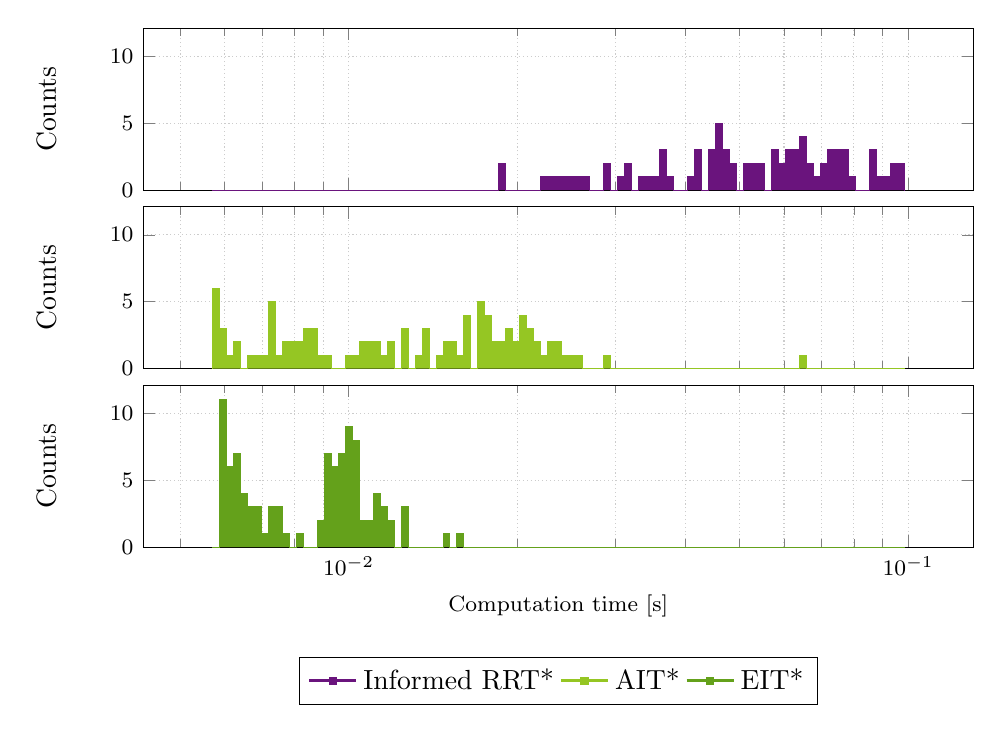
\begin{tikzpicture} [
  xscale=1,
  yscale=1
]
\begin{axis} [
  width=\textwidth,
  height=0.3\textwidth,
  at={(0cm, 0cm)},
  unbounded coords=jump,
  xtick align=inside,
  ytick align=inside,
  axis line style={solid, black},
  name=defaultInformedRRTstarISDPA,
  xmajorgrids,
  xminorgrids,
  ymajorgrids,
  major grid style={densely dotted, black!20},
  minor grid style={densely dotted, black!20},
  ymin=0,
  ymax=11,
  enlarge y limits=upper,
  xmode=log,
  xlabel={{\empty}},
  xlabel style={font=\footnotesize},
  xticklabel={{\empty}},
  xticklabel style={font=\footnotesize},
  ylabel={Counts},
  ylabel style={font=\footnotesize, text depth=0.0em, text height=0.5em},
  ylabel absolute,
  yticklabel style={font=\footnotesize}
]
\addplot [
  line width=0,
  color=pdtpurple,
  mark="none",
  const plot,
  name path={defaultInformedRRTstarInitialSolutionDurationHistogram},
  fill=pdtpurple
] table [
  row sep=\\,
  col sep=&
]{
0.00570601 & 0\\
0.00570601 & 0\\
0.00587252 & 0\\
0.0060439 & 0\\
0.00622027 & 0\\
0.00640179 & 0\\
0.00658861 & 0\\
0.00678089 & 0\\
0.00697877 & 0\\
0.00718243 & 0\\
0.00739203 & 0\\
0.00760774 & 0\\
0.00782975 & 0\\
0.00805825 & 0\\
0.0082934 & 0\\
0.00853543 & 0\\
0.00878451 & 0\\
0.00904086 & 0\\
0.0093047 & 0\\
0.00957623 & 0\\
0.00985569 & 0\\
0.0101433 & 0\\
0.0104393 & 0\\
0.0107439 & 0\\
0.0110575 & 0\\
0.0113802 & 0\\
0.0117123 & 0\\
0.0120541 & 0\\
0.0124058 & 0\\
0.0127679 & 0\\
0.0131405 & 0\\
0.0135239 & 0\\
0.0139186 & 0\\
0.0143248 & 0\\
0.0147428 & 0\\
0.015173 & 0\\
0.0156158 & 0\\
0.0160715 & 0\\
0.0165405 & 0\\
0.0170232 & 0\\
0.01752 & 0\\
0.0180313 & 0\\
0.0185575 & 2\\
0.019099 & 0\\
0.0196564 & 0\\
0.02023 & 0\\
0.0208203 & 0\\
0.0214279 & 0\\
0.0220532 & 1\\
0.0226968 & 1\\
0.0233592 & 1\\
0.0240408 & 1\\
0.0247424 & 1\\
0.0254644 & 1\\
0.0262076 & 1\\
0.0269724 & 0\\
0.0277595 & 0\\
0.0285696 & 2\\
0.0294033 & 0\\
0.0302613 & 1\\
0.0311444 & 2\\
0.0320533 & 0\\
0.0329887 & 1\\
0.0339514 & 1\\
0.0349422 & 1\\
0.0359619 & 3\\
0.0370113 & 1\\
0.0380914 & 0\\
0.039203 & 0\\
0.040347 & 1\\
0.0415245 & 3\\
0.0427362 & 0\\
0.0439834 & 3\\
0.0452669 & 5\\
0.0465879 & 3\\
0.0479475 & 2\\
0.0493467 & 0\\
0.0507867 & 2\\
0.0522688 & 2\\
0.0537941 & 2\\
0.055364 & 0\\
0.0569796 & 3\\
0.0586424 & 2\\
0.0603538 & 3\\
0.062115 & 3\\
0.0639277 & 4\\
0.0657933 & 2\\
0.0677133 & 1\\
0.0696893 & 2\\
0.071723 & 3\\
0.073816 & 3\\
0.0759702 & 3\\
0.0781872 & 1\\
0.0804688 & 0\\
0.0828171 & 0\\
0.0852339 & 3\\
0.0877213 & 1\\
0.0902812 & 1\\
0.0929158 & 2\\
0.0956273 & 2\\
0.0984179 & 0\\
0.0984179 & 0\\
};

\end{axis}

\begin{axis} [
  width=\textwidth,
  height=0.3\textwidth,
  at={($(defaultInformedRRTstarISDPA.south) - (0.0em, 0.6em)$)},
  unbounded coords=jump,
  xtick align=inside,
  ytick align=inside,
  axis line style={solid, black},
  name=defaultAITstarISDPA,
  anchor=north,
  xmajorgrids,
  xminorgrids,
  ymajorgrids,
  major grid style={densely dotted, black!20},
  minor grid style={densely dotted, black!20},
  ymin=0,
  ymax=11,
  enlarge y limits=upper,
  xmode=log,
  xlabel={{\empty}},
  xlabel style={font=\footnotesize},
  xticklabel={{\empty}},
  xticklabel style={font=\footnotesize},
  ylabel={Counts},
  ylabel style={font=\footnotesize, text depth=0.0em, text height=0.5em},
  ylabel absolute,
  yticklabel style={font=\footnotesize}
]
\addplot [
  line width=0,
  color=pdtlightgreen,
  mark="none",
  const plot,
  name path={defaultAITstarInitialSolutionDurationHistogram},
  fill=pdtlightgreen
] table [
  row sep=\\,
  col sep=&
]{
0.00570601 & 0\\
0.00570601 & 6\\
0.00587252 & 3\\
0.0060439 & 1\\
0.00622027 & 2\\
0.00640179 & 0\\
0.00658861 & 1\\
0.00678089 & 1\\
0.00697877 & 1\\
0.00718243 & 5\\
0.00739203 & 1\\
0.00760774 & 2\\
0.00782975 & 2\\
0.00805825 & 2\\
0.0082934 & 3\\
0.00853543 & 3\\
0.00878451 & 1\\
0.00904086 & 1\\
0.0093047 & 0\\
0.00957623 & 0\\
0.00985569 & 1\\
0.0101433 & 1\\
0.0104393 & 2\\
0.0107439 & 2\\
0.0110575 & 2\\
0.0113802 & 1\\
0.0117123 & 2\\
0.0120541 & 0\\
0.0124058 & 3\\
0.0127679 & 0\\
0.0131405 & 1\\
0.0135239 & 3\\
0.0139186 & 0\\
0.0143248 & 1\\
0.0147428 & 2\\
0.015173 & 2\\
0.0156158 & 1\\
0.0160715 & 4\\
0.0165405 & 0\\
0.0170232 & 5\\
0.01752 & 4\\
0.0180313 & 2\\
0.0185575 & 2\\
0.019099 & 3\\
0.0196564 & 2\\
0.02023 & 4\\
0.0208203 & 3\\
0.0214279 & 2\\
0.0220532 & 1\\
0.0226968 & 2\\
0.0233592 & 2\\
0.0240408 & 1\\
0.0247424 & 1\\
0.0254644 & 1\\
0.0262076 & 0\\
0.0269724 & 0\\
0.0277595 & 0\\
0.0285696 & 1\\
0.0294033 & 0\\
0.0302613 & 0\\
0.0311444 & 0\\
0.0320533 & 0\\
0.0329887 & 0\\
0.0339514 & 0\\
0.0349422 & 0\\
0.0359619 & 0\\
0.0370113 & 0\\
0.0380914 & 0\\
0.039203 & 0\\
0.040347 & 0\\
0.0415245 & 0\\
0.0427362 & 0\\
0.0439834 & 0\\
0.0452669 & 0\\
0.0465879 & 0\\
0.0479475 & 0\\
0.0493467 & 0\\
0.0507867 & 0\\
0.0522688 & 0\\
0.0537941 & 0\\
0.055364 & 0\\
0.0569796 & 0\\
0.0586424 & 0\\
0.0603538 & 0\\
0.062115 & 0\\
0.0639277 & 1\\
0.0657933 & 0\\
0.0677133 & 0\\
0.0696893 & 0\\
0.071723 & 0\\
0.073816 & 0\\
0.0759702 & 0\\
0.0781872 & 0\\
0.0804688 & 0\\
0.0828171 & 0\\
0.0852339 & 0\\
0.0877213 & 0\\
0.0902812 & 0\\
0.0929158 & 0\\
0.0956273 & 0\\
0.0984179 & 0\\
0.0984179 & 0\\
};

\end{axis}

\begin{axis} [
  width=\textwidth,
  height=0.3\textwidth,
  at={($(defaultAITstarISDPA.south) - (0.0em, 0.6em)$)},
  unbounded coords=jump,
  xtick align=inside,
  ytick align=inside,
  axis line style={solid, black},
  name=defaultEITstarISDPA,
  anchor=north,
  xmajorgrids,
  xminorgrids,
  ymajorgrids,
  major grid style={densely dotted, black!20},
  minor grid style={densely dotted, black!20},
  ymin=0,
  ymax=11,
  enlarge y limits=upper,
  xmode=log,
  xlabel={Computation time [s]},
  xlabel style={font=\footnotesize},
  xticklabel style={font=\footnotesize},
  ylabel={Counts},
  ylabel style={font=\footnotesize, text depth=0.0em, text height=0.5em},
  ylabel absolute,
  yticklabel style={font=\footnotesize}
]
\addplot [
  line width=0,
  color=pdtgreen,
  mark="none",
  const plot,
  name path={defaultEITstarInitialSolutionDurationHistogram},
  fill=pdtgreen
] table [
  row sep=\\,
  col sep=&
]{
0.00570601 & 0\\
0.00570601 & 0\\
0.00587252 & 11\\
0.0060439 & 6\\
0.00622027 & 7\\
0.00640179 & 4\\
0.00658861 & 3\\
0.00678089 & 3\\
0.00697877 & 1\\
0.00718243 & 3\\
0.00739203 & 3\\
0.00760774 & 1\\
0.00782975 & 0\\
0.00805825 & 1\\
0.0082934 & 0\\
0.00853543 & 0\\
0.00878451 & 2\\
0.00904086 & 7\\
0.0093047 & 6\\
0.00957623 & 7\\
0.00985569 & 9\\
0.0101433 & 8\\
0.0104393 & 2\\
0.0107439 & 2\\
0.0110575 & 4\\
0.0113802 & 3\\
0.0117123 & 2\\
0.0120541 & 0\\
0.0124058 & 3\\
0.0127679 & 0\\
0.0131405 & 0\\
0.0135239 & 0\\
0.0139186 & 0\\
0.0143248 & 0\\
0.0147428 & 1\\
0.015173 & 0\\
0.0156158 & 1\\
0.0160715 & 0\\
0.0165405 & 0\\
0.0170232 & 0\\
0.01752 & 0\\
0.0180313 & 0\\
0.0185575 & 0\\
0.019099 & 0\\
0.0196564 & 0\\
0.02023 & 0\\
0.0208203 & 0\\
0.0214279 & 0\\
0.0220532 & 0\\
0.0226968 & 0\\
0.0233592 & 0\\
0.0240408 & 0\\
0.0247424 & 0\\
0.0254644 & 0\\
0.0262076 & 0\\
0.0269724 & 0\\
0.0277595 & 0\\
0.0285696 & 0\\
0.0294033 & 0\\
0.0302613 & 0\\
0.0311444 & 0\\
0.0320533 & 0\\
0.0329887 & 0\\
0.0339514 & 0\\
0.0349422 & 0\\
0.0359619 & 0\\
0.0370113 & 0\\
0.0380914 & 0\\
0.039203 & 0\\
0.040347 & 0\\
0.0415245 & 0\\
0.0427362 & 0\\
0.0439834 & 0\\
0.0452669 & 0\\
0.0465879 & 0\\
0.0479475 & 0\\
0.0493467 & 0\\
0.0507867 & 0\\
0.0522688 & 0\\
0.0537941 & 0\\
0.055364 & 0\\
0.0569796 & 0\\
0.0586424 & 0\\
0.0603538 & 0\\
0.062115 & 0\\
0.0639277 & 0\\
0.0657933 & 0\\
0.0677133 & 0\\
0.0696893 & 0\\
0.071723 & 0\\
0.073816 & 0\\
0.0759702 & 0\\
0.0781872 & 0\\
0.0804688 & 0\\
0.0828171 & 0\\
0.0852339 & 0\\
0.0877213 & 0\\
0.0902812 & 0\\
0.0929158 & 0\\
0.0956273 & 0\\
0.0984179 & 0\\
0.0984179 & 0\\
};

\end{axis}

\begin{axis} [
  width=\textwidth,
  height=0.5\textwidth,
  at={($(defaultEITstarISDPA.south) - (0.0em, 0.6em)$)},
  unbounded coords=jump,
  xtick align=inside,
  ytick align=inside,
  axis line style={solid, black},
  anchor=north,
  hide axis,
  xmajorgrids,
  ymajorgrids,
  major grid style={densely dotted, black!20},
  xmin=0,
  xmax=10,
  ymin=0,
  ymax=10,
  xlabel style={font=\footnotesize},
  xticklabel style={font=\footnotesize},
  ylabel style={font=\footnotesize},
  yticklabel style={font=\footnotesize},
  legend style={anchor=south, legend cell align=left, legend columns=-1, at={(axis cs:5, 6)}}
]
\addlegendimage{pdtpurple, line width = 1.0pt, mark size=1.0pt, mark=square*}
\addlegendentry{Informed RRT*}
\addlegendimage{pdtlightgreen, line width = 1.0pt, mark size=1.0pt, mark=square*}
\addlegendentry{AIT*}
\addlegendimage{pdtgreen, line width = 1.0pt, mark size=1.0pt, mark=square*}
\addlegendentry{EIT*}
\end{axis}

\end{tikzpicture}%
\captionof{figure}{\footnotesize Histograms of initial solution times.}
\end{center}
\pagebreak
\section{Informed HZ}\label{sec:defaultInformedHZ}
\subsection{Initial Solutions}\label{sec:defaultInformedHZ-initial-solution}
\begin{center}
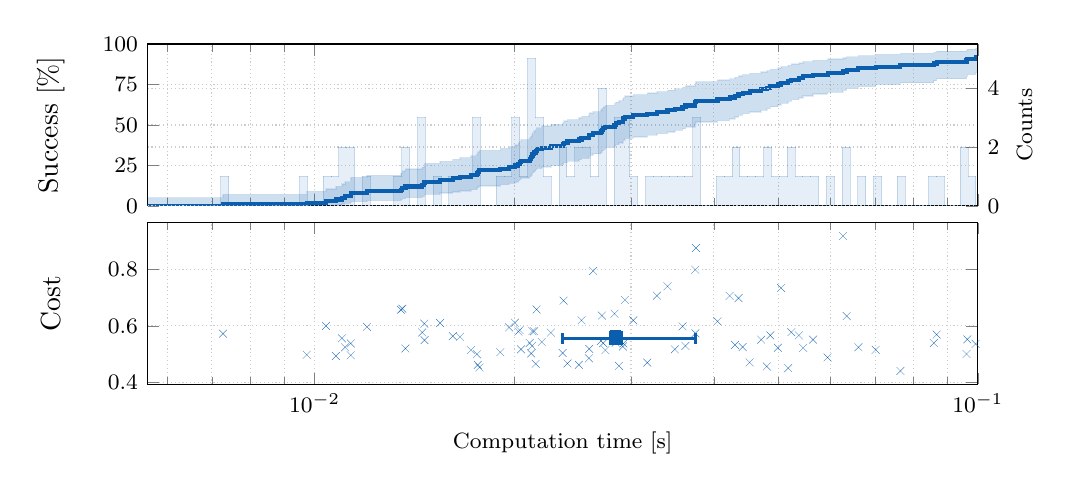
\begin{tikzpicture} [
  xscale=1,
  yscale=1
]
\begin{axis} [
  width=\textwidth,
  height=0.3\textwidth,
  at={(0cm, 0cm)},
  unbounded coords=jump,
  xtick align=inside,
  ytick align=inside,
  axis line style={solid, black},
  name=SuccessAxis,
  xmajorgrids,
  xminorgrids,
  ymajorgrids,
  major grid style={densely dotted, black!20},
  minor grid style={densely dotted, black!20},
  xmin=0.00727877,
  xmax=0.1,
  enlarge x limits=lower,
  ymin=0,
  ymax=100,
  xmode=log,
  xlabel={{\empty}},
  xlabel style={font=\footnotesize},
  xticklabel={{\empty}},
  xticklabel style={font=\footnotesize},
  ylabel={Success [\%]},
  ylabel style={font=\footnotesize, text depth=0.0em, text height=0.5em},
  ylabel absolute,
  ytick={0,25,50,75,100},
 ytick pos={left},
  yticklabel style={font=\footnotesize}
]
\addplot [
  line width=0.5,
  color=pdtblue,
  mark="none",
  const plot,
  name path={defaultInformedHZSuccessUpperConfidence},
  fill opacity=0.2,
  draw opacity=0.1
] table [
  row sep=\\,
  col sep=&
]{
1e-09 & 5.1604\\
0.00727877 & 7.19577\\
0.00973225 & 8.94307\\
0.0104066 & 10.5481\\
0.0107682 & 12.0633\\
0.010999 & 13.5145\\
0.0111162 & 14.9169\\
0.0113376 & 16.2803\\
0.0113403 & 17.6114\\
0.0119951 & 18.9152\\
0.013495 & 20.1954\\
0.0135649 & 21.4547\\
0.013711 & 22.6955\\
0.0145303 & 23.9196\\
0.0146348 & 25.1285\\
0.0146493 & 26.3235\\
0.0154656 & 27.5057\\
0.0161594 & 28.676\\
0.0165704 & 29.8351\\
0.0172065 & 30.9838\\
0.0175742 & 32.1226\\
0.0176248 & 33.2522\\
0.0177204 & 34.3729\\
0.0190552 & 35.4851\\
0.0196488 & 36.5893\\
0.0200467 & 37.6857\\
0.0202887 & 38.7747\\
0.020381 & 39.8566\\
0.0204754 & 40.9315\\
0.0211006 & 41.9997\\
0.0212063 & 43.0614\\
0.0212722 & 44.1167\\
0.0213053 & 45.1659\\
0.0214283 & 46.2091\\
0.0215501 & 47.2464\\
0.0216166 & 48.2779\\
0.022005 & 49.3038\\
0.0227139 & 50.3241\\
0.0236598 & 51.339\\
0.0237366 & 52.3485\\
0.0240574 & 53.3527\\
0.0250324 & 54.3517\\
0.0252641 & 55.3454\\
0.0259226 & 56.3341\\
0.0259509 & 57.3177\\
0.0263047 & 58.2962\\
0.0270289 & 59.2697\\
0.0271227 & 60.2382\\
0.0272447 & 61.2017\\
0.0274476 & 62.1603\\
0.0283301 & 63.1139\\
0.0284432 & 64.0625\\
0.0287661 & 65.0062\\
0.0291703 & 65.9449\\
0.0292128 & 66.8786\\
0.0293656 & 67.8073\\
0.0302357 & 68.7309\\
0.0317436 & 69.6495\\
0.0328258 & 70.5629\\
0.0340542 & 71.4712\\
0.0349318 & 72.3742\\
0.0358798 & 73.272\\
0.0362481 & 74.1644\\
0.0374956 & 75.0513\\
0.0375168 & 75.9327\\
0.0375791 & 76.8085\\
0.0405042 & 77.6785\\
0.0422518 & 78.5426\\
0.0430411 & 79.4008\\
0.0435778 & 80.2528\\
0.0442043 & 81.0985\\
0.045286 & 81.9378\\
0.0471368 & 82.7703\\
0.0480712 & 83.596\\
0.0486525 & 84.4145\\
0.0499548 & 85.2256\\
0.0505113 & 86.0291\\
0.0517676 & 86.8245\\
0.0523413 & 87.6116\\
0.0537283 & 88.3899\\
0.0545338 & 89.1589\\
0.056435 & 89.9183\\
0.0593674 & 90.6673\\
0.062623 & 91.4053\\
0.0634351 & 92.1315\\
0.0660638 & 92.8452\\
0.0701477 & 93.5451\\
0.0764454 & 94.2303\\
0.0858301 & 94.8991\\
0.0867008 & 95.5498\\
0.0961613 & 96.1804\\
0.0964124 & 96.7882\\
0.0992366 & 97.3699\\
0.105796 & 97.3699\\
};

\addplot [
  line width=0.5,
  color=pdtblue,
  mark="none",
  const plot,
  name path={defaultInformedHZSuccessLowerConfidence},
  fill opacity=0.2,
  draw opacity=0.1
] table [
  row sep=\\,
  col sep=&
]{
1e-09 & 0\\
0.00727877 & 0.00501242\\
0.00973225 & 0.103962\\
0.0104066 & 0.340707\\
0.0107682 & 0.680169\\
0.010999 & 1.09403\\
0.0111162 & 1.56425\\
0.0113376 & 2.07899\\
0.0113403 & 2.63012\\
0.0119951 & 3.21176\\
0.013495 & 3.81957\\
0.0135649 & 4.45017\\
0.013711 & 5.10094\\
0.0145303 & 5.76975\\
0.0146348 & 6.45486\\
0.0146493 & 7.15483\\
0.0154656 & 7.86846\\
0.0161594 & 8.59473\\
0.0165704 & 9.33274\\
0.0172065 & 10.0817\\
0.0175742 & 10.8411\\
0.0176248 & 11.6101\\
0.0177204 & 12.3884\\
0.0190552 & 13.1755\\
0.0196488 & 13.9709\\
0.0200467 & 14.7744\\
0.0202887 & 15.5855\\
0.020381 & 16.404\\
0.0204754 & 17.2297\\
0.0211006 & 18.0622\\
0.0212063 & 18.9015\\
0.0212722 & 19.7472\\
0.0213053 & 20.5992\\
0.0214283 & 21.4574\\
0.0215501 & 22.3215\\
0.0216166 & 23.1915\\
0.022005 & 24.0673\\
0.0227139 & 24.9487\\
0.0236598 & 25.8356\\
0.0237366 & 26.728\\
0.0240574 & 27.6258\\
0.0250324 & 28.5288\\
0.0252641 & 29.4371\\
0.0259226 & 30.3505\\
0.0259509 & 31.2691\\
0.0263047 & 32.1927\\
0.0270289 & 33.1214\\
0.0271227 & 34.0551\\
0.0272447 & 34.9938\\
0.0274476 & 35.9375\\
0.0283301 & 36.8861\\
0.0284432 & 37.8397\\
0.0287661 & 38.7983\\
0.0291703 & 39.7618\\
0.0292128 & 40.7303\\
0.0293656 & 41.7038\\
0.0302357 & 42.6823\\
0.0317436 & 43.6659\\
0.0328258 & 44.6546\\
0.0340542 & 45.6483\\
0.0349318 & 46.6473\\
0.0358798 & 47.6515\\
0.0362481 & 48.661\\
0.0374956 & 49.6759\\
0.0375168 & 50.6962\\
0.0375791 & 51.7221\\
0.0405042 & 52.7536\\
0.0422518 & 53.7909\\
0.0430411 & 54.8341\\
0.0435778 & 55.8833\\
0.0442043 & 56.9386\\
0.045286 & 58.0003\\
0.0471368 & 59.0685\\
0.0480712 & 60.1434\\
0.0486525 & 61.2253\\
0.0499548 & 62.3143\\
0.0505113 & 63.4107\\
0.0517676 & 64.5149\\
0.0523413 & 65.6271\\
0.0537283 & 66.7478\\
0.0545338 & 67.8774\\
0.056435 & 69.0162\\
0.0593674 & 70.1649\\
0.062623 & 71.324\\
0.0634351 & 72.4943\\
0.0660638 & 73.6765\\
0.0701477 & 74.8715\\
0.0764454 & 76.0804\\
0.0858301 & 77.3045\\
0.0867008 & 78.5453\\
0.0961613 & 79.8046\\
0.0964124 & 81.0848\\
0.0992366 & 82.3886\\
0.105796 & 82.3886\\
};

\addplot [
  line width=1,
  color=pdtblue,
  mark=square*,
  mark size=2,
  const plot,
  fill opacity=0.2,
  draw opacity=0
] fill between [
  of =defaultInformedHZSuccessUpperConfidence and defaultInformedHZSuccessLowerConfidence
];
\addplot [
  line width=1.5,
  color=pdtblue,
  mark="none",
  const plot,
  name path={defaultInformedHZSuccess}
] table [
  row sep=\\,
  col sep=&
]{
1e-09 & 0\\
0.00727877 & 1\\
0.00973225 & 2\\
0.0104066 & 3\\
0.0107682 & 4\\
0.010999 & 5\\
0.0111162 & 6\\
0.0113376 & 7\\
0.0113403 & 8\\
0.0119951 & 9\\
0.013495 & 10\\
0.0135649 & 11\\
0.013711 & 12\\
0.0145303 & 13\\
0.0146348 & 14\\
0.0146493 & 15\\
0.0154656 & 16\\
0.0161594 & 17\\
0.0165704 & 18\\
0.0172065 & 19\\
0.0175742 & 20\\
0.0176248 & 21\\
0.0177204 & 22\\
0.0190552 & 23\\
0.0196488 & 24\\
0.0200467 & 25\\
0.0202887 & 26\\
0.020381 & 27\\
0.0204754 & 28\\
0.0211006 & 29\\
0.0212063 & 30\\
0.0212722 & 31\\
0.0213053 & 32\\
0.0214283 & 33\\
0.0215501 & 34\\
0.0216166 & 35\\
0.022005 & 36\\
0.0227139 & 37\\
0.0236598 & 38\\
0.0237366 & 39\\
0.0240574 & 40\\
0.0250324 & 41\\
0.0252641 & 42\\
0.0259226 & 43\\
0.0259509 & 44\\
0.0263047 & 45\\
0.0270289 & 46\\
0.0271227 & 47\\
0.0272447 & 48\\
0.0274476 & 49\\
0.0283301 & 50\\
0.0284432 & 51\\
0.0287661 & 52\\
0.0291703 & 53\\
0.0292128 & 54\\
0.0293656 & 55\\
0.0302357 & 56\\
0.0317436 & 57\\
0.0328258 & 58\\
0.0340542 & 59\\
0.0349318 & 60\\
0.0358798 & 61\\
0.0362481 & 62\\
0.0374956 & 63\\
0.0375168 & 64\\
0.0375791 & 65\\
0.0405042 & 66\\
0.0422518 & 67\\
0.0430411 & 68\\
0.0435778 & 69\\
0.0442043 & 70\\
0.045286 & 71\\
0.0471368 & 72\\
0.0480712 & 73\\
0.0486525 & 74\\
0.0499548 & 75\\
0.0505113 & 76\\
0.0517676 & 77\\
0.0523413 & 78\\
0.0537283 & 79\\
0.0545338 & 80\\
0.056435 & 81\\
0.0593674 & 82\\
0.062623 & 83\\
0.0634351 & 84\\
0.0660638 & 85\\
0.0701477 & 86\\
0.0764454 & 87\\
0.0858301 & 88\\
0.0867008 & 89\\
0.0961613 & 90\\
0.0964124 & 91\\
0.0992366 & 92\\
0.105796 & 92\\
};

\end{axis}

\begin{axis} [
  width=\textwidth,
  height=0.3\textwidth,
  at={(0cm, 0cm)},
  unbounded coords=jump,
  xtick align=inside,
  ytick align=inside,
  axis line style={solid, black},
  name=defaultInformedHZISDPA,
  xmajorgrids,
  xminorgrids,
  ymajorgrids,
  major grid style={densely dotted, black!20},
  minor grid style={densely dotted, black!20},
  xmin=0.00727877,
  xmax=0.1,
  enlarge x limits=lower,
  ymin=0,
  ymax=5,
  enlarge y limits=upper,
  xmode=log,
  axis x line=none,
  axis y line*=right,
  xlabel={Computation time [s]},
  xlabel style={font=\footnotesize},
  xtick={{\empty}},
  xticklabel={{\empty}},
  xticklabel style={font=\footnotesize},
  ylabel={Counts},
  ylabel style={font=\footnotesize, text depth=0.0em, text height=0.5em},
  yticklabel style={font=\footnotesize}
]
\addplot [
  line width=0,
  color=pdtblue,
  mark="none",
  const plot,
  name path={defaultInformedHZInitialSolutionDurationHistogram},
  fill=pdtblue,
  fill opacity=0.1,
  draw opacity=0.2
] table [
  row sep=\\,
  col sep=&
]{
0.00665587 & 0\\
0.00665587 & 0\\
0.00684012 & 0\\
0.00702946 & 0\\
0.00722404 & 1\\
0.00742401 & 0\\
0.00762951 & 0\\
0.00784071 & 0\\
0.00805775 & 0\\
0.00828079 & 0\\
0.00851002 & 0\\
0.00874558 & 0\\
0.00898767 & 0\\
0.00923646 & 0\\
0.00949213 & 1\\
0.00975488 & 0\\
0.0100249 & 0\\
0.0103024 & 1\\
0.0105876 & 1\\
0.0108807 & 2\\
0.0111819 & 2\\
0.0114914 & 0\\
0.0118095 & 1\\
0.0121364 & 0\\
0.0124723 & 0\\
0.0128176 & 0\\
0.0131724 & 1\\
0.013537 & 2\\
0.0139117 & 0\\
0.0142968 & 3\\
0.0146926 & 0\\
0.0150993 & 1\\
0.0155172 & 0\\
0.0159468 & 1\\
0.0163882 & 1\\
0.0168418 & 1\\
0.017308 & 3\\
0.0177871 & 0\\
0.0182795 & 0\\
0.0187855 & 1\\
0.0193055 & 1\\
0.0198399 & 3\\
0.0203891 & 1\\
0.0209535 & 5\\
0.0215335 & 3\\
0.0221296 & 1\\
0.0227421 & 0\\
0.0233717 & 2\\
0.0240186 & 1\\
0.0246835 & 2\\
0.0253667 & 2\\
0.0260689 & 1\\
0.0267905 & 4\\
0.0275321 & 0\\
0.0282942 & 3\\
0.0290774 & 3\\
0.0298823 & 1\\
0.0307095 & 0\\
0.0315596 & 1\\
0.0324332 & 1\\
0.033331 & 1\\
0.0342536 & 1\\
0.0352018 & 1\\
0.0361762 & 1\\
0.0371776 & 3\\
0.0382067 & 0\\
0.0392643 & 0\\
0.0403512 & 1\\
0.0414682 & 1\\
0.042616 & 2\\
0.0437957 & 1\\
0.045008 & 1\\
0.0462539 & 1\\
0.0475342 & 2\\
0.04885 & 1\\
0.0502023 & 1\\
0.0515919 & 2\\
0.05302 & 1\\
0.0544877 & 1\\
0.055996 & 1\\
0.057546 & 0\\
0.0591389 & 1\\
0.0607759 & 0\\
0.0624583 & 2\\
0.0641872 & 0\\
0.065964 & 1\\
0.0677899 & 0\\
0.0696664 & 1\\
0.0715949 & 0\\
0.0735767 & 0\\
0.0756134 & 1\\
0.0777064 & 0\\
0.0798574 & 0\\
0.082068 & 0\\
0.0843397 & 1\\
0.0866743 & 1\\
0.0890735 & 0\\
0.0915392 & 0\\
0.0940731 & 2\\
0.0966771 & 1\\
0.0993532 & 0\\
0.0993532 & 0\\
};

\end{axis}

\begin{axis} [
  width=\textwidth,
  height=0.3\textwidth,
  at={($(SuccessAxis.south) - (0.0em, 0.6em)$)},
  unbounded coords=jump,
  xtick align=inside,
  ytick align=inside,
  axis line style={solid, black},
  name=defaultInformedHZInitialSolutionScatterAxis,
  anchor=north,
  xmajorgrids,
  xminorgrids,
  ymajorgrids,
  major grid style={densely dotted, black!20},
  minor grid style={densely dotted, black!20},
  xmin=0.00727877,
  xmax=0.1,
  enlarge x limits=lower,
  xmode=log,
  xlabel={Computation time [s]},
  xlabel style={font=\footnotesize},
  xticklabel style={font=\footnotesize},
  ylabel={Cost},
  ylabel style={font=\footnotesize, text depth=0.0em, text height=0.5em},
  ylabel absolute,
  yticklabel style={font=\footnotesize}
]
\addplot [
  line width=0.1,
  color=pdtblue,
  mark=x,
  mark size=2,
  only marks,
  name path={defaultInformedHZInitialSolutionScatterPlotlineWidth}
] table [
  row sep=\\,
  col sep=&
]{
0.0545338 & 0.522418\\
0.0964124 & 0.552523\\
0.0505113 & 0.733975\\
0.0177204 & 0.453609\\
0.0430411 & 0.533024\\
0.0240574 & 0.467611\\
0.0215501 & 0.466251\\
0.0113376 & 0.496435\\
0.0660638 & 0.524903\\
0.0537283 & 0.56672\\
0.0292128 & 0.537986\\
0.0701477 & 0.515575\\
0.0263047 & 0.794084\\
0.0202887 & 0.57989\\
0.0593674 & 0.488696\\
0.0237366 & 0.689022\\
0.0213053 & 0.58157\\
0.062623 & 0.917277\\
0.0252641 & 0.620054\\
0.0287661 & 0.45923\\
0.013495 & 0.657134\\
0.0284432 & 0.540848\\
0.0992366 & 0.536446\\
0.0250324 & 0.46275\\
0.0212063 & 0.502645\\
0.0375168 & 0.573969\\
0.0362481 & 0.529306\\
0.0214283 & 0.58092\\
0.0154656 & 0.610325\\
0.0764454 & 0.441048\\
inf & inf\\
0.0227139 & 0.576249\\
inf & inf\\
0.0236598 & 0.504591\\
0.0135649 & 0.660626\\
0.013711 & 0.520386\\
0.0212722 & 0.529119\\
0.0111162 & 0.524367\\
0.056435 & 0.551736\\
0.010999 & 0.556215\\
0.0271227 & 0.636556\\
0.0119951 & 0.596862\\
0.045286 & 0.471206\\
0.00973225 & 0.498141\\
0.0274476 & 0.51443\\
0.0328258 & 0.706615\\
inf & inf\\
0.0471368 & 0.551296\\
0.020381 & 0.585022\\
0.0499548 & 0.522901\\
0.0422518 & 0.705923\\
0.0146493 & 0.54991\\
0.0317436 & 0.470478\\
0.0165704 & 0.561789\\
0.0196488 & 0.594682\\
inf & inf\\
0.0291703 & 0.52732\\
0.0634351 & 0.634716\\
0.0146348 & 0.60782\\
0.0480712 & 0.457042\\
0.0375791 & 0.875036\\
0.0340542 & 0.739939\\
0.0200467 & 0.611343\\
0.0104066 & 0.600178\\
0.0283301 & 0.642834\\
0.00727877 & 0.572739\\
0.0272447 & 0.53937\\
0.0259226 & 0.485403\\
0.0961613 & 0.500826\\
0.0523413 & 0.577879\\
0.0176248 & 0.462521\\
0.0867008 & 0.5696\\
0.0145303 & 0.577043\\
0.0858301 & 0.539373\\
0.0113403 & 0.538233\\
0.0349318 & 0.517383\\
0.0175742 & 0.499715\\
0.0216166 & 0.658085\\
0.0204754 & 0.517087\\
0.0107682 & 0.493909\\
0.0259509 & 0.519052\\
0.0172065 & 0.514625\\
0.0190552 & 0.50716\\
0.0293656 & 0.691929\\
0.0270289 & 0.546921\\
0.0486525 & 0.566674\\
inf & inf\\
inf & inf\\
0.0358798 & 0.598686\\
0.0374956 & 0.798258\\
0.0405042 & 0.61631\\
inf & inf\\
0.0302357 & 0.619746\\
0.0442043 & 0.52546\\
0.0435778 & 0.698113\\
0.0517676 & 0.450729\\
0.0211006 & 0.539897\\
inf & inf\\
0.0161594 & 0.563993\\
0.022005 & 0.543072\\
};

\addplot [
  line width=1,
  color=pdtblue,
  mark=square*,
  mark size=2,
  only marks,
  const plot,
  name path={defaultInformedHZMedianInitialSolution}
] table [
  row sep=\\,
  col sep=&
]{
0.0284432 & 0.556215\\
};

\addplot [
  line width=1,
  color=pdtblue,
  mark=|,
  mark size=2,
  const plot,
  name path={defaultInformedHZMedianInitialSolutionDurationConfidenceInterval}
] table [
  row sep=\\,
  col sep=&
]{
0.0236598 & 0.556215\\
0.0375168 & 0.556215\\
};

\addplot [
  line width=1,
  color=pdtblue,
  mark=-,
  mark size=2,
  const plot,
  name path={defaultInformedHZMedianInitialSolutionDurationConfidenceInterval}
] table [
  row sep=\\,
  col sep=&
]{
0.0284432 & 0.536446\\
0.0284432 & 0.58157\\
};

\end{axis}

\end{tikzpicture}%
\captionof{figure}{\footnotesize \textbf{Top:} Histogram and associated empirical distribution function (EDF) of Informed HZ with a Clopper-Pearson (nonparametric) 99\% confidence interval for the underlying CDF. \textbf{Bottom:} All initial solutions of Informed HZ and their median with a nonparametric 99\% confidence interval.}
\end{center}
\subsection{Cost Evolution}\label{sec:defaultInformedHZ-cost-evolution}
\begin{center}
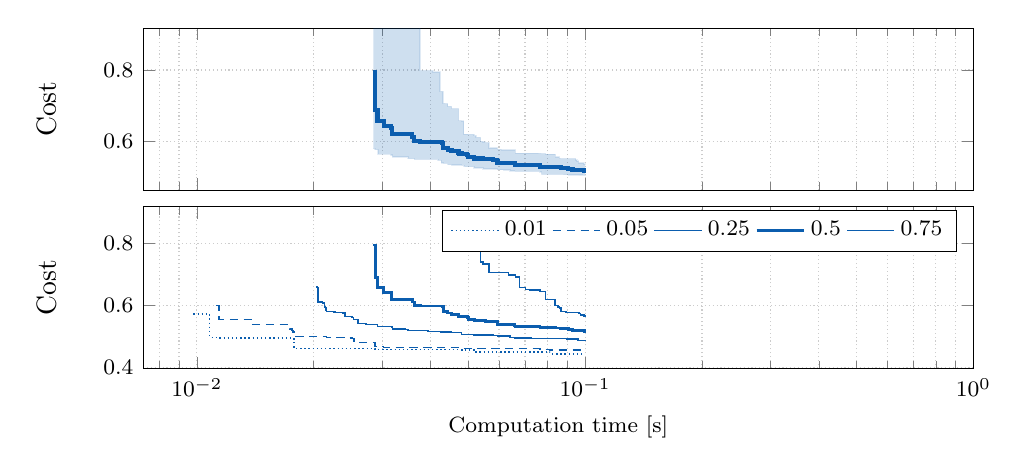
\begin{tikzpicture} [
  xscale=1,
  yscale=1
]
\begin{axis} [
  width=\textwidth,
  height=0.3\textwidth,
  at={(0cm, 0cm)},
  unbounded coords=jump,
  xtick align=inside,
  ytick align=inside,
  axis line style={solid, black},
  name=defaultInformedHZMedianCostAxis,
  xmajorgrids,
  xminorgrids,
  ymajorgrids,
  major grid style={densely dotted, black!20},
  minor grid style={densely dotted, black!20},
  xmin=0.00727877,
  xmax=1,
  ymax=0.917277,
  xmode=log,
  xlabel={{\empty}},
  xlabel style={font=\footnotesize},
  xticklabel={{\empty}},
  xticklabel style={font=\footnotesize},
  ylabel={Cost},
  ylabel style={font=\footnotesize, text depth=0.0em, text height=0.5em},
  ylabel absolute,
  yticklabel style={font=\footnotesize}
]
\addplot [
  line width=0.5,
  color=pdtblue,
  mark="none",
  const plot,
  name path={defaultInformedHZMedianCostEvolutionUpperConfidence},
  fill opacity=0.2,
  draw opacity=0.1
] table [
  row sep=\\,
  col sep=&
]{
0.0285 & 2.75183\\
0.0375 & 2.75183\\
0.0376 & 0.798258\\
0.0405 & 0.798258\\
0.0406 & 0.794084\\
0.0422 & 0.794084\\
0.0423 & 0.739939\\
0.043 & 0.739939\\
0.0431 & 0.706615\\
0.0435 & 0.706615\\
0.0436 & 0.705923\\
0.0442 & 0.705923\\
0.0443 & 0.698113\\
0.0452 & 0.698113\\
0.0453 & 0.691929\\
0.0471 & 0.691929\\
0.0472 & 0.658085\\
0.048 & 0.658085\\
0.0481 & 0.657134\\
0.0486 & 0.657134\\
0.0487 & 0.620054\\
0.0499 & 0.620054\\
0.05 & 0.619746\\
0.0517 & 0.619746\\
0.0518 & 0.61631\\
0.0523 & 0.61631\\
0.0524 & 0.611343\\
0.0537 & 0.611343\\
0.0538 & 0.600178\\
0.0545 & 0.600178\\
0.0546 & 0.598686\\
0.0552 & 0.598686\\
0.0553 & 0.596429\\
0.0564 & 0.596429\\
0.0565 & 0.58157\\
0.0593 & 0.58157\\
0.0594 & 0.577879\\
0.0609 & 0.577879\\
0.061 & 0.576081\\
0.066 & 0.576081\\
0.0661 & 0.56672\\
0.0701 & 0.56672\\
0.0702 & 0.566717\\
0.0756 & 0.566717\\
0.0757 & 0.56671\\
0.0758 & 0.566682\\
0.0759 & 0.566674\\
0.0764 & 0.566674\\
0.0765 & 0.566673\\
0.077 & 0.566673\\
0.0771 & 0.565966\\
0.079 & 0.565966\\
0.0791 & 0.563993\\
0.0837 & 0.563993\\
0.0838 & 0.556215\\
0.0858 & 0.556215\\
0.0859 & 0.552257\\
0.0864 & 0.552257\\
0.0865 & 0.55181\\
0.0926 & 0.55181\\
0.0927 & 0.551736\\
0.0945 & 0.551736\\
0.0946 & 0.547667\\
0.0951 & 0.547667\\
0.0952 & 0.544896\\
0.0961 & 0.544896\\
0.0962 & 0.539373\\
0.0992 & 0.539373\\
0.0993 & 0.536932\\
0.0994 & 0.536446\\
0.0999 & 0.536446\\
0.1 & 0.536446\\
};

\addplot [
  line width=0.5,
  color=pdtblue,
  mark="none",
  const plot,
  name path={defaultInformedHZMedianCostEvolutionLowerConfidence},
  fill opacity=0.2,
  draw opacity=0.1
] table [
  row sep=\\,
  col sep=&
]{
0.0285 & 0.57989\\
0.0287 & 0.57989\\
0.0288 & 0.577043\\
0.0291 & 0.577043\\
0.0292 & 0.576249\\
0.0293 & 0.563993\\
0.0314 & 0.563993\\
0.0315 & 0.563041\\
0.0316 & 0.561789\\
0.0317 & 0.561789\\
0.0318 & 0.560175\\
0.0319 & 0.556215\\
0.0349 & 0.556215\\
0.035 & 0.55181\\
0.0362 & 0.55181\\
0.0363 & 0.54964\\
0.0417 & 0.54964\\
0.0418 & 0.546921\\
0.0425 & 0.546921\\
0.0426 & 0.539897\\
0.0429 & 0.539897\\
0.043 & 0.53937\\
0.0431 & 0.538233\\
0.0432 & 0.537986\\
0.0442 & 0.537986\\
0.0443 & 0.534868\\
0.0452 & 0.534868\\
0.0453 & 0.533555\\
0.048 & 0.533555\\
0.0481 & 0.533024\\
0.0487 & 0.533024\\
0.0488 & 0.530883\\
0.0489 & 0.529306\\
0.0499 & 0.529306\\
0.05 & 0.529119\\
0.0517 & 0.529119\\
0.0518 & 0.52546\\
0.0545 & 0.52546\\
0.0546 & 0.522901\\
0.0577 & 0.522901\\
0.0578 & 0.522418\\
0.0593 & 0.522418\\
0.0594 & 0.520386\\
0.0616 & 0.520386\\
0.0617 & 0.519575\\
0.0639 & 0.519575\\
0.064 & 0.517087\\
0.0658 & 0.517087\\
0.0659 & 0.516025\\
0.0701 & 0.516025\\
0.0702 & 0.515683\\
0.0733 & 0.515683\\
0.0734 & 0.515575\\
0.0764 & 0.515575\\
0.0765 & 0.51443\\
0.0771 & 0.51443\\
0.0772 & 0.510899\\
0.0773 & 0.507983\\
0.0774 & 0.50716\\
0.0878 & 0.50716\\
0.0879 & 0.507109\\
0.0904 & 0.507109\\
0.0905 & 0.505948\\
0.0927 & 0.505948\\
0.0928 & 0.505837\\
0.0961 & 0.505837\\
0.0962 & 0.505274\\
0.0985 & 0.505274\\
0.0986 & 0.505138\\
0.0994 & 0.505138\\
0.0995 & 0.504591\\
0.0999 & 0.504591\\
0.1 & 0.504591\\
};

\addplot [
  line width=1,
  color=pdtblue,
  mark=square*,
  mark size=2,
  const plot,
  fill opacity=0.2,
  draw opacity=0
] fill between [
  of =defaultInformedHZMedianCostEvolutionUpperConfidence and defaultInformedHZMedianCostEvolutionLowerConfidence
];
\addplot [
  line width=1.5,
  color=pdtblue,
  mark="none",
  const plot,
  name path={defaultInformedHZMedianCostEvolution}
] table [
  row sep=\\,
  col sep=&
]{
0.0001 & inf\\
0.0284 & inf\\
0.0285 & 0.794084\\
0.0287 & 0.794084\\
0.0288 & 0.689022\\
0.0291 & 0.689022\\
0.0292 & 0.658085\\
0.0293 & 0.657134\\
0.0302 & 0.657134\\
0.0303 & 0.642834\\
0.0316 & 0.642834\\
0.0317 & 0.636556\\
0.0318 & 0.620054\\
0.0349 & 0.620054\\
0.035 & 0.619746\\
0.0358 & 0.619746\\
0.0359 & 0.611343\\
0.0362 & 0.611343\\
0.0363 & 0.600178\\
0.0375 & 0.600178\\
0.0376 & 0.598686\\
0.0428 & 0.598686\\
0.0429 & 0.596429\\
0.043 & 0.596429\\
0.0431 & 0.58157\\
0.0442 & 0.58157\\
0.0443 & 0.576081\\
0.0452 & 0.576081\\
0.0453 & 0.572326\\
0.0471 & 0.572326\\
0.0472 & 0.566717\\
0.0473 & 0.565966\\
0.048 & 0.565966\\
0.0481 & 0.563993\\
0.0496 & 0.563993\\
0.0497 & 0.561193\\
0.0499 & 0.561193\\
0.05 & 0.556215\\
0.0517 & 0.556215\\
0.0518 & 0.55181\\
0.0545 & 0.55181\\
0.0546 & 0.551296\\
0.0553 & 0.551296\\
0.0554 & 0.54964\\
0.0577 & 0.54964\\
0.0578 & 0.547667\\
0.0593 & 0.547667\\
0.0594 & 0.54416\\
0.0595 & 0.53937\\
0.0638 & 0.53937\\
0.0639 & 0.538233\\
0.0658 & 0.538233\\
0.0659 & 0.534419\\
0.066 & 0.534419\\
0.0661 & 0.533807\\
0.0701 & 0.533807\\
0.0702 & 0.533555\\
0.0746 & 0.533555\\
0.0747 & 0.533438\\
0.0748 & 0.532999\\
0.0764 & 0.532999\\
0.0765 & 0.529306\\
0.0771 & 0.529306\\
0.0772 & 0.529119\\
0.0837 & 0.529119\\
0.0838 & 0.527665\\
0.0865 & 0.527665\\
0.0866 & 0.52546\\
0.0904 & 0.52546\\
0.0905 & 0.522901\\
0.0927 & 0.522901\\
0.0928 & 0.520386\\
0.0946 & 0.520386\\
0.0947 & 0.519937\\
0.0961 & 0.519937\\
0.0962 & 0.519575\\
0.0994 & 0.519575\\
0.0995 & 0.517447\\
0.0999 & 0.517447\\
0.1 & 0.517447\\
};

\end{axis}

\begin{axis} [
  width=\textwidth,
  height=0.3\textwidth,
  at={($(defaultInformedHZMedianCostAxis.south) - (0.0em, 0.6em)$)},
  unbounded coords=jump,
  xtick align=inside,
  ytick align=inside,
  axis line style={solid, black},
  name=defaultInformedHZCostPercentileEvolutionAxis,
  anchor=north,
  xmajorgrids,
  xminorgrids,
  ymajorgrids,
  major grid style={densely dotted, black!20},
  minor grid style={densely dotted, black!20},
  xmin=0.00727877,
  xmax=1,
  ymax=0.917277,
  xmode=log,
  xlabel={Computation time [s]},
  xlabel style={font=\footnotesize},
  xticklabel style={font=\footnotesize},
  ylabel={Cost},
  ylabel style={font=\footnotesize, text depth=0.0em, text height=0.5em},
  ylabel absolute,
  yticklabel style={font=\footnotesize},
  legend style={font=\footnotesize, legend cell align=left, legend columns=-1}
]
\addplot [
  line width=0.5,
  color=pdtblue,
  mark="none",
  const plot,
  densely dotted,
  name path={defaultInformedHZpercentile0.01CostEvolution}
] table [
  row sep=\\,
  col sep=&
]{
0.0001 & inf\\
0.0097 & inf\\
0.0098 & 0.572739\\
0.0107 & 0.572739\\
0.0108 & 0.498141\\
0.0113 & 0.498141\\
0.0114 & 0.496435\\
0.0176 & 0.496435\\
0.0177 & 0.493909\\
0.0178 & 0.462521\\
0.0287 & 0.462521\\
0.0288 & 0.45923\\
0.048 & 0.45923\\
0.0481 & 0.457042\\
0.0517 & 0.457042\\
0.0518 & 0.451428\\
0.0764 & 0.451428\\
0.0765 & 0.450729\\
0.081 & 0.450729\\
0.0811 & 0.444802\\
0.0999 & 0.444802\\
0.1 & 0.444802\\
};
\addlegendentry{0.01}

\addplot [
  line width=0.5,
  color=pdtblue,
  mark="none",
  const plot,
  densely dashed,
  name path={defaultInformedHZpercentile0.05CostEvolution}
] table [
  row sep=\\,
  col sep=&
]{
0.0001 & inf\\
0.0111 & inf\\
0.0112 & 0.600178\\
0.0113 & 0.600178\\
0.0114 & 0.556215\\
0.0137 & 0.556215\\
0.0138 & 0.538233\\
0.0172 & 0.538233\\
0.0173 & 0.524367\\
0.0175 & 0.524367\\
0.0176 & 0.520386\\
0.0177 & 0.514625\\
0.0178 & 0.499715\\
0.0215 & 0.499715\\
0.0216 & 0.498141\\
0.024 & 0.498141\\
0.0241 & 0.496435\\
0.025 & 0.496435\\
0.0251 & 0.493909\\
0.0253 & 0.493909\\
0.0254 & 0.482368\\
0.0287 & 0.482368\\
0.0288 & 0.467611\\
0.0302 & 0.467611\\
0.0303 & 0.466251\\
0.048 & 0.466251\\
0.0481 & 0.46275\\
0.0517 & 0.46275\\
0.0518 & 0.462521\\
0.0617 & 0.462521\\
0.0618 & 0.461963\\
0.0764 & 0.461963\\
0.0765 & 0.45923\\
0.0809 & 0.45923\\
0.081 & 0.457042\\
0.0999 & 0.457042\\
0.1 & 0.457042\\
};
\addlegendentry{0.05}

\addplot [
  line width=0.5,
  color=pdtblue,
  mark="none",
  const plot,
  name path={defaultInformedHZpercentile0.25CostEvolution}
] table [
  row sep=\\,
  col sep=&
]{
0.0001 & inf\\
0.0202 & inf\\
0.0203 & 0.660626\\
0.0204 & 0.657134\\
0.0205 & 0.611343\\
0.021 & 0.611343\\
0.0211 & 0.60782\\
0.0212 & 0.60782\\
0.0213 & 0.596862\\
0.0214 & 0.594682\\
0.0215 & 0.585022\\
0.0216 & 0.58157\\
0.022 & 0.58157\\
0.0221 & 0.58092\\
0.0224 & 0.58092\\
0.0225 & 0.57989\\
0.0227 & 0.57989\\
0.0228 & 0.577043\\
0.0236 & 0.577043\\
0.0237 & 0.576249\\
0.024 & 0.576249\\
0.0241 & 0.563993\\
0.025 & 0.563993\\
0.0251 & 0.561789\\
0.0252 & 0.561789\\
0.0253 & 0.556215\\
0.0259 & 0.556215\\
0.026 & 0.543072\\
0.0272 & 0.543072\\
0.0273 & 0.539897\\
0.0274 & 0.539897\\
0.0275 & 0.53937\\
0.0287 & 0.53937\\
0.0288 & 0.538233\\
0.0291 & 0.538233\\
0.0292 & 0.533555\\
0.0317 & 0.533555\\
0.0318 & 0.529119\\
0.0319 & 0.524367\\
0.0344 & 0.524367\\
0.0345 & 0.522217\\
0.0349 & 0.522217\\
0.035 & 0.520386\\
0.0393 & 0.520386\\
0.0394 & 0.517855\\
0.0395 & 0.517383\\
0.0419 & 0.517383\\
0.042 & 0.517087\\
0.0424 & 0.517087\\
0.0425 & 0.515683\\
0.0432 & 0.515683\\
0.0433 & 0.514625\\
0.0452 & 0.514625\\
0.0453 & 0.51443\\
0.048 & 0.51443\\
0.0481 & 0.50716\\
0.0517 & 0.50716\\
0.0518 & 0.505948\\
0.0526 & 0.505948\\
0.0527 & 0.505837\\
0.0544 & 0.505837\\
0.0545 & 0.505138\\
0.0578 & 0.505138\\
0.0579 & 0.504591\\
0.0593 & 0.504591\\
0.0594 & 0.502645\\
0.0616 & 0.502645\\
0.0617 & 0.502598\\
0.0639 & 0.502598\\
0.064 & 0.497197\\
0.0659 & 0.497197\\
0.066 & 0.496435\\
0.0727 & 0.496435\\
0.0728 & 0.494569\\
0.0731 & 0.494569\\
0.0732 & 0.494517\\
0.0733 & 0.49429\\
0.0734 & 0.494206\\
0.0735 & 0.493985\\
0.0764 & 0.493985\\
0.0765 & 0.493909\\
0.0894 & 0.493909\\
0.0895 & 0.493562\\
0.0896 & 0.493272\\
0.0905 & 0.493272\\
0.0906 & 0.492096\\
0.0958 & 0.492096\\
0.0959 & 0.488696\\
0.0999 & 0.488696\\
0.1 & 0.488696\\
};
\addlegendentry{0.25}

\addplot [
  line width=1,
  color=pdtblue,
  mark="none",
  const plot,
  name path={defaultInformedHZpercentile0.5CostEvolution}
] table [
  row sep=\\,
  col sep=&
]{
0.0001 & inf\\
0.0284 & inf\\
0.0285 & 0.794084\\
0.0287 & 0.794084\\
0.0288 & 0.689022\\
0.0291 & 0.689022\\
0.0292 & 0.658085\\
0.0293 & 0.657134\\
0.0302 & 0.657134\\
0.0303 & 0.642834\\
0.0316 & 0.642834\\
0.0317 & 0.636556\\
0.0318 & 0.620054\\
0.0349 & 0.620054\\
0.035 & 0.619746\\
0.0358 & 0.619746\\
0.0359 & 0.611343\\
0.0362 & 0.611343\\
0.0363 & 0.600178\\
0.0375 & 0.600178\\
0.0376 & 0.598686\\
0.0428 & 0.598686\\
0.0429 & 0.596429\\
0.043 & 0.596429\\
0.0431 & 0.58157\\
0.0442 & 0.58157\\
0.0443 & 0.576081\\
0.0452 & 0.576081\\
0.0453 & 0.572326\\
0.0471 & 0.572326\\
0.0472 & 0.566717\\
0.0473 & 0.565966\\
0.048 & 0.565966\\
0.0481 & 0.563993\\
0.0496 & 0.563993\\
0.0497 & 0.561193\\
0.0499 & 0.561193\\
0.05 & 0.556215\\
0.0517 & 0.556215\\
0.0518 & 0.55181\\
0.0545 & 0.55181\\
0.0546 & 0.551296\\
0.0553 & 0.551296\\
0.0554 & 0.54964\\
0.0577 & 0.54964\\
0.0578 & 0.547667\\
0.0593 & 0.547667\\
0.0594 & 0.54416\\
0.0595 & 0.53937\\
0.0638 & 0.53937\\
0.0639 & 0.538233\\
0.0658 & 0.538233\\
0.0659 & 0.534419\\
0.066 & 0.534419\\
0.0661 & 0.533807\\
0.0701 & 0.533807\\
0.0702 & 0.533555\\
0.0746 & 0.533555\\
0.0747 & 0.533438\\
0.0748 & 0.532999\\
0.0764 & 0.532999\\
0.0765 & 0.529306\\
0.0771 & 0.529306\\
0.0772 & 0.529119\\
0.0837 & 0.529119\\
0.0838 & 0.527665\\
0.0865 & 0.527665\\
0.0866 & 0.52546\\
0.0904 & 0.52546\\
0.0905 & 0.522901\\
0.0927 & 0.522901\\
0.0928 & 0.520386\\
0.0946 & 0.520386\\
0.0947 & 0.519937\\
0.0961 & 0.519937\\
0.0962 & 0.519575\\
0.0994 & 0.519575\\
0.0995 & 0.517447\\
0.0999 & 0.517447\\
0.1 & 0.517447\\
};
\addlegendentry{0.5}

\addplot [
  line width=0.5,
  color=pdtblue,
  mark="none",
  const plot,
  name path={defaultInformedHZpercentile0.75CostEvolution}
] table [
  row sep=\\,
  col sep=&
]{
0.0001 & inf\\
0.0505 & inf\\
0.0506 & 0.875036\\
0.0517 & 0.875036\\
0.0518 & 0.798258\\
0.0523 & 0.798258\\
0.0524 & 0.794084\\
0.0537 & 0.794084\\
0.0538 & 0.739939\\
0.0545 & 0.739939\\
0.0546 & 0.733975\\
0.0564 & 0.733975\\
0.0565 & 0.706615\\
0.0593 & 0.706615\\
0.0594 & 0.705923\\
0.0634 & 0.705923\\
0.0635 & 0.698113\\
0.066 & 0.698113\\
0.0661 & 0.691929\\
0.0676 & 0.691929\\
0.0677 & 0.658085\\
0.0686 & 0.658085\\
0.0687 & 0.657718\\
0.0688 & 0.657134\\
0.0701 & 0.657134\\
0.0702 & 0.650584\\
0.0717 & 0.650584\\
0.0718 & 0.65029\\
0.0764 & 0.65029\\
0.0765 & 0.644854\\
0.0789 & 0.644854\\
0.079 & 0.64035\\
0.0791 & 0.620054\\
0.0836 & 0.620054\\
0.0837 & 0.600178\\
0.085 & 0.600178\\
0.0851 & 0.595419\\
0.0858 & 0.595419\\
0.0859 & 0.592575\\
0.0866 & 0.592575\\
0.0867 & 0.58157\\
0.0892 & 0.58157\\
0.0893 & 0.577336\\
0.0961 & 0.577336\\
0.0962 & 0.576081\\
0.0964 & 0.576081\\
0.0965 & 0.574521\\
0.0972 & 0.574521\\
0.0973 & 0.57042\\
0.0974 & 0.5696\\
0.0992 & 0.5696\\
0.0993 & 0.56672\\
0.0999 & 0.56672\\
0.1 & 0.56672\\
};
\addlegendentry{0.75}

\addplot [
  line width=0.5,
  color=pdtblue,
  mark="none",
  const plot,
  densely dashed,
  name path={defaultInformedHZpercentile0.95CostEvolution}
] table [
  row sep=\\,
  col sep=&
]{
0.0001 & inf\\
0.0999 & inf\\
0.1 & inf\\
};
\addlegendentry{0.95}

\addplot [
  line width=0.5,
  color=pdtblue,
  mark="none",
  const plot,
  densely dotted,
  name path={defaultInformedHZpercentile0.99CostEvolution}
] table [
  row sep=\\,
  col sep=&
]{
0.0001 & inf\\
0.0999 & inf\\
0.1 & inf\\
};
\addlegendentry{0.99}

\end{axis}

\end{tikzpicture}%
\captionof{figure}{\footnotesize \textbf{Top:} Median cost evolution of Informed HZ with a nonparametric 99\% confidence interval. \textbf{Bottom:} Seven percentiles of the cost evolution of Informed HZ.}\end{center}

\pagebreak
\section{Informed RRT*}\label{sec:defaultInformedRRTstar}
\subsection{Initial Solutions}\label{sec:defaultInformedRRTstar-initial-solution}
\begin{center}
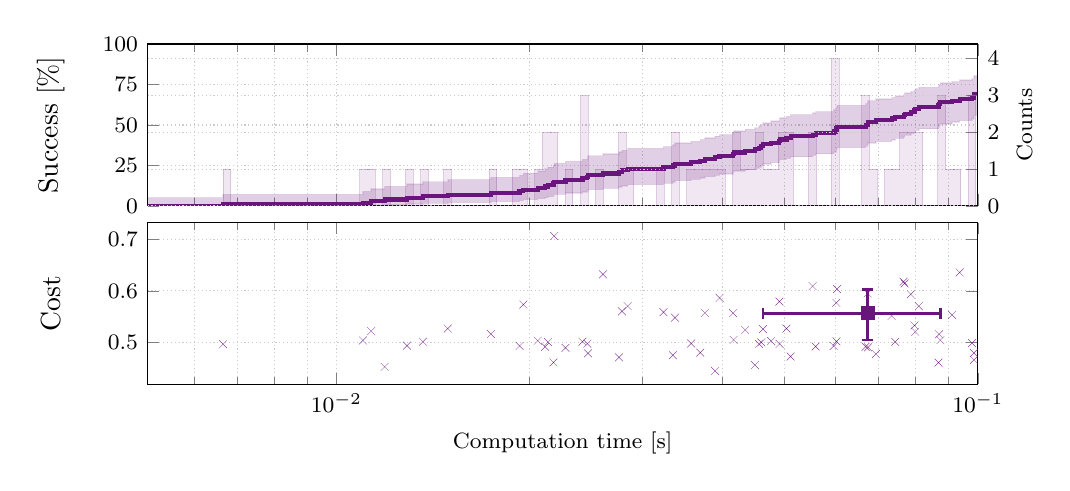
\begin{tikzpicture} [
  xscale=1,
  yscale=1
]
\begin{axis} [
  width=\textwidth,
  height=0.3\textwidth,
  at={(0cm, 0cm)},
  unbounded coords=jump,
  xtick align=inside,
  ytick align=inside,
  axis line style={solid, black},
  name=SuccessAxis,
  xmajorgrids,
  xminorgrids,
  ymajorgrids,
  major grid style={densely dotted, black!20},
  minor grid style={densely dotted, black!20},
  xmin=0.00665588,
  xmax=0.1,
  enlarge x limits=lower,
  ymin=0,
  ymax=100,
  xmode=log,
  xlabel={{\empty}},
  xlabel style={font=\footnotesize},
  xticklabel={{\empty}},
  xticklabel style={font=\footnotesize},
  ylabel={Success [\%]},
  ylabel style={font=\footnotesize, text depth=0.0em, text height=0.5em},
  ylabel absolute,
  ytick={0,25,50,75,100},
 ytick pos={left},
  yticklabel style={font=\footnotesize}
]
\addplot [
  line width=0.5,
  color=pdtpurple,
  mark="none",
  const plot,
  name path={defaultInformedRRTstarSuccessUpperConfidence},
  fill opacity=0.2,
  draw opacity=0.1
] table [
  row sep=\\,
  col sep=&
]{
1e-09 & 5.1604\\
0.00665588 & 7.19577\\
0.0109981 & 8.94307\\
0.0113252 & 10.5481\\
0.0118879 & 12.0633\\
0.012885 & 13.5145\\
0.0136406 & 14.9169\\
0.0149167 & 16.2803\\
0.0174142 & 17.6114\\
0.0192996 & 18.9152\\
0.0195611 & 20.1954\\
0.0205997 & 21.4547\\
0.0211507 & 22.6955\\
0.0213788 & 23.9196\\
0.0217959 & 25.1285\\
0.0218553 & 26.3235\\
0.0227563 & 27.5057\\
0.0241851 & 28.676\\
0.0246132 & 29.8351\\
0.0246751 & 30.9838\\
0.026039 & 32.1226\\
0.0275755 & 33.2522\\
0.027874 & 34.3729\\
0.0284468 & 35.4851\\
0.0323495 & 36.5893\\
0.0334627 & 37.6857\\
0.0337192 & 38.7747\\
0.0357377 & 39.8566\\
0.0369242 & 40.9315\\
0.0375449 & 41.9997\\
0.0389398 & 43.0614\\
0.0395695 & 44.1167\\
0.0415413 & 45.1659\\
0.0416202 & 46.2091\\
0.0433862 & 47.2464\\
0.0449325 & 48.2779\\
0.0455861 & 49.3038\\
0.0459696 & 50.3241\\
0.0462543 & 51.339\\
0.0476233 & 52.3485\\
0.0490496 & 53.3527\\
0.0490832 & 54.3517\\
0.0503102 & 55.3454\\
0.051061 & 56.3341\\
0.0552754 & 57.3177\\
0.0558574 & 58.2962\\
0.0596094 & 59.2697\\
0.060168 & 60.2382\\
0.0602102 & 61.2017\\
0.0603232 & 62.1603\\
0.0668468 & 63.1139\\
0.0673452 & 64.0625\\
0.0674193 & 65.0062\\
0.0693535 & 65.9449\\
0.0733934 & 66.8786\\
0.0743694 & 67.8073\\
0.0766362 & 68.7309\\
0.0769146 & 69.6495\\
0.0786418 & 70.5629\\
0.0796633 & 71.4712\\
0.0798913 & 72.3742\\
0.0809224 & 73.272\\
0.0868428 & 74.1644\\
0.0870175 & 75.0513\\
0.087436 & 75.9327\\
0.09117 & 76.8085\\
0.093708 & 77.6785\\
0.0979317 & 78.5426\\
0.0986167 & 79.4008\\
0.0986649 & 80.2528\\
0.102103 & 81.0985\\
0.105796 & 81.0985\\
};

\addplot [
  line width=0.5,
  color=pdtpurple,
  mark="none",
  const plot,
  name path={defaultInformedRRTstarSuccessLowerConfidence},
  fill opacity=0.2,
  draw opacity=0.1
] table [
  row sep=\\,
  col sep=&
]{
1e-09 & 0\\
0.00665588 & 0.00501242\\
0.0109981 & 0.103962\\
0.0113252 & 0.340707\\
0.0118879 & 0.680169\\
0.012885 & 1.09403\\
0.0136406 & 1.56425\\
0.0149167 & 2.07899\\
0.0174142 & 2.63012\\
0.0192996 & 3.21176\\
0.0195611 & 3.81957\\
0.0205997 & 4.45017\\
0.0211507 & 5.10094\\
0.0213788 & 5.76975\\
0.0217959 & 6.45486\\
0.0218553 & 7.15483\\
0.0227563 & 7.86846\\
0.0241851 & 8.59473\\
0.0246132 & 9.33274\\
0.0246751 & 10.0817\\
0.026039 & 10.8411\\
0.0275755 & 11.6101\\
0.027874 & 12.3884\\
0.0284468 & 13.1755\\
0.0323495 & 13.9709\\
0.0334627 & 14.7744\\
0.0337192 & 15.5855\\
0.0357377 & 16.404\\
0.0369242 & 17.2297\\
0.0375449 & 18.0622\\
0.0389398 & 18.9015\\
0.0395695 & 19.7472\\
0.0415413 & 20.5992\\
0.0416202 & 21.4574\\
0.0433862 & 22.3215\\
0.0449325 & 23.1915\\
0.0455861 & 24.0673\\
0.0459696 & 24.9487\\
0.0462543 & 25.8356\\
0.0476233 & 26.728\\
0.0490496 & 27.6258\\
0.0490832 & 28.5288\\
0.0503102 & 29.4371\\
0.051061 & 30.3505\\
0.0552754 & 31.2691\\
0.0558574 & 32.1927\\
0.0596094 & 33.1214\\
0.060168 & 34.0551\\
0.0602102 & 34.9938\\
0.0603232 & 35.9375\\
0.0668468 & 36.8861\\
0.0673452 & 37.8397\\
0.0674193 & 38.7983\\
0.0693535 & 39.7618\\
0.0733934 & 40.7303\\
0.0743694 & 41.7038\\
0.0766362 & 42.6823\\
0.0769146 & 43.6659\\
0.0786418 & 44.6546\\
0.0796633 & 45.6483\\
0.0798913 & 46.6473\\
0.0809224 & 47.6515\\
0.0868428 & 48.661\\
0.0870175 & 49.6759\\
0.087436 & 50.6962\\
0.09117 & 51.7221\\
0.093708 & 52.7536\\
0.0979317 & 53.7909\\
0.0986167 & 54.8341\\
0.0986649 & 55.8833\\
0.102103 & 56.9386\\
0.105796 & 56.9386\\
};

\addplot [
  line width=1,
  color=pdtpurple,
  mark=square*,
  mark size=2,
  const plot,
  fill opacity=0.2,
  draw opacity=0
] fill between [
  of =defaultInformedRRTstarSuccessUpperConfidence and defaultInformedRRTstarSuccessLowerConfidence
];
\addplot [
  line width=1.5,
  color=pdtpurple,
  mark="none",
  const plot,
  name path={defaultInformedRRTstarSuccess}
] table [
  row sep=\\,
  col sep=&
]{
1e-09 & 0\\
0.00665588 & 1\\
0.0109981 & 2\\
0.0113252 & 3\\
0.0118879 & 4\\
0.012885 & 5\\
0.0136406 & 6\\
0.0149167 & 7\\
0.0174142 & 8\\
0.0192996 & 9\\
0.0195611 & 10\\
0.0205997 & 11\\
0.0211507 & 12\\
0.0213788 & 13\\
0.0217959 & 14\\
0.0218553 & 15\\
0.0227563 & 16\\
0.0241851 & 17\\
0.0246132 & 18\\
0.0246751 & 19\\
0.026039 & 20\\
0.0275755 & 21\\
0.027874 & 22\\
0.0284468 & 23\\
0.0323495 & 24\\
0.0334627 & 25\\
0.0337192 & 26\\
0.0357377 & 27\\
0.0369242 & 28\\
0.0375449 & 29\\
0.0389398 & 30\\
0.0395695 & 31\\
0.0415413 & 32\\
0.0416202 & 33\\
0.0433862 & 34\\
0.0449325 & 35\\
0.0455861 & 36\\
0.0459696 & 37\\
0.0462543 & 38\\
0.0476233 & 39\\
0.0490496 & 40\\
0.0490832 & 41\\
0.0503102 & 42\\
0.051061 & 43\\
0.0552754 & 44\\
0.0558574 & 45\\
0.0596094 & 46\\
0.060168 & 47\\
0.0602102 & 48\\
0.0603232 & 49\\
0.0668468 & 50\\
0.0673452 & 51\\
0.0674193 & 52\\
0.0693535 & 53\\
0.0733934 & 54\\
0.0743694 & 55\\
0.0766362 & 56\\
0.0769146 & 57\\
0.0786418 & 58\\
0.0796633 & 59\\
0.0798913 & 60\\
0.0809224 & 61\\
0.0868428 & 62\\
0.0870175 & 63\\
0.087436 & 64\\
0.09117 & 65\\
0.093708 & 66\\
0.0979317 & 67\\
0.0986167 & 68\\
0.0986649 & 69\\
0.102103 & 70\\
0.105796 & 70\\
};

\end{axis}

\begin{axis} [
  width=\textwidth,
  height=0.3\textwidth,
  at={(0cm, 0cm)},
  unbounded coords=jump,
  xtick align=inside,
  ytick align=inside,
  axis line style={solid, black},
  name=defaultInformedRRTstarISDPA,
  xmajorgrids,
  xminorgrids,
  ymajorgrids,
  major grid style={densely dotted, black!20},
  minor grid style={densely dotted, black!20},
  xmin=0.00665588,
  xmax=0.1,
  enlarge x limits=lower,
  ymin=0,
  ymax=4,
  enlarge y limits=upper,
  xmode=log,
  axis x line=none,
  axis y line*=right,
  xlabel={Computation time [s]},
  xlabel style={font=\footnotesize},
  xtick={{\empty}},
  xticklabel={{\empty}},
  xticklabel style={font=\footnotesize},
  ylabel={Counts},
  ylabel style={font=\footnotesize, text depth=0.0em, text height=0.5em},
  yticklabel style={font=\footnotesize}
]
\addplot [
  line width=0,
  color=pdtpurple,
  mark="none",
  const plot,
  name path={defaultInformedRRTstarInitialSolutionDurationHistogram},
  fill=pdtpurple,
  fill opacity=0.1,
  draw opacity=0.2
] table [
  row sep=\\,
  col sep=&
]{
0.00665587 & 0\\
0.00665587 & 1\\
0.00684012 & 0\\
0.00702946 & 0\\
0.00722404 & 0\\
0.00742401 & 0\\
0.00762951 & 0\\
0.00784071 & 0\\
0.00805775 & 0\\
0.00828079 & 0\\
0.00851002 & 0\\
0.00874558 & 0\\
0.00898767 & 0\\
0.00923646 & 0\\
0.00949213 & 0\\
0.00975488 & 0\\
0.0100249 & 0\\
0.0103024 & 0\\
0.0105876 & 0\\
0.0108807 & 1\\
0.0111819 & 1\\
0.0114914 & 0\\
0.0118095 & 1\\
0.0121364 & 0\\
0.0124723 & 0\\
0.0128176 & 1\\
0.0131724 & 0\\
0.013537 & 1\\
0.0139117 & 0\\
0.0142968 & 0\\
0.0146926 & 1\\
0.0150993 & 0\\
0.0155172 & 0\\
0.0159468 & 0\\
0.0163882 & 0\\
0.0168418 & 0\\
0.017308 & 1\\
0.0177871 & 0\\
0.0182795 & 0\\
0.0187855 & 1\\
0.0193055 & 1\\
0.0198399 & 0\\
0.0203891 & 1\\
0.0209535 & 2\\
0.0215335 & 2\\
0.0221296 & 0\\
0.0227421 & 1\\
0.0233717 & 0\\
0.0240186 & 3\\
0.0246835 & 0\\
0.0253667 & 1\\
0.0260689 & 0\\
0.0267905 & 0\\
0.0275321 & 2\\
0.0282942 & 1\\
0.0290774 & 0\\
0.0298823 & 0\\
0.0307095 & 0\\
0.0315596 & 1\\
0.0324332 & 0\\
0.033331 & 2\\
0.0342536 & 0\\
0.0352018 & 1\\
0.0361762 & 1\\
0.0371776 & 1\\
0.0382067 & 1\\
0.0392643 & 1\\
0.0403512 & 0\\
0.0414682 & 2\\
0.042616 & 1\\
0.0437957 & 1\\
0.045008 & 2\\
0.0462539 & 1\\
0.0475342 & 1\\
0.04885 & 2\\
0.0502023 & 2\\
0.0515919 & 0\\
0.05302 & 0\\
0.0544877 & 2\\
0.055996 & 0\\
0.057546 & 0\\
0.0591389 & 4\\
0.0607759 & 0\\
0.0624583 & 0\\
0.0641872 & 0\\
0.065964 & 3\\
0.0677899 & 1\\
0.0696664 & 0\\
0.0715949 & 1\\
0.0735767 & 1\\
0.0756134 & 2\\
0.0777064 & 2\\
0.0798574 & 2\\
0.082068 & 0\\
0.0843397 & 0\\
0.0866743 & 3\\
0.0890735 & 1\\
0.0915392 & 1\\
0.0940731 & 0\\
0.0966771 & 3\\
0.0993532 & 0\\
0.0993532 & 0\\
};

\end{axis}

\begin{axis} [
  width=\textwidth,
  height=0.3\textwidth,
  at={($(SuccessAxis.south) - (0.0em, 0.6em)$)},
  unbounded coords=jump,
  xtick align=inside,
  ytick align=inside,
  axis line style={solid, black},
  name=defaultInformedRRTstarInitialSolutionScatterAxis,
  anchor=north,
  xmajorgrids,
  xminorgrids,
  ymajorgrids,
  major grid style={densely dotted, black!20},
  minor grid style={densely dotted, black!20},
  xmin=0.00665588,
  xmax=0.1,
  enlarge x limits=lower,
  xmode=log,
  xlabel={Computation time [s]},
  xlabel style={font=\footnotesize},
  xticklabel style={font=\footnotesize},
  ylabel={Cost},
  ylabel style={font=\footnotesize, text depth=0.0em, text height=0.5em},
  ylabel absolute,
  yticklabel style={font=\footnotesize}
]
\addplot [
  line width=0.1,
  color=pdtpurple,
  mark=x,
  mark size=2,
  only marks,
  name path={defaultInformedRRTstarInitialSolutionScatterPlotlineWidth}
] table [
  row sep=\\,
  col sep=&
]{
inf & inf\\
0.0786418 & 0.593369\\
0.0868428 & 0.460671\\
0.0375449 & 0.557342\\
0.0192996 & 0.493002\\
0.0136406 & 0.501277\\
0.0246132 & 0.497526\\
inf & inf\\
0.0217959 & 0.460868\\
0.0227563 & 0.489312\\
inf & inf\\
0.0389398 & 0.444428\\
inf & inf\\
0.012885 & 0.493719\\
0.0979317 & 0.498458\\
inf & inf\\
0.0334627 & 0.474954\\
0.0769146 & 0.614502\\
0.0357377 & 0.49779\\
inf & inf\\
inf & inf\\
0.051061 & 0.472474\\
inf & inf\\
0.060168 & 0.576959\\
0.0433862 & 0.524031\\
0.0174142 & 0.516163\\
0.0476233 & 0.50254\\
0.027874 & 0.560338\\
0.0798913 & 0.520627\\
0.087436 & 0.504322\\
inf & inf\\
0.0462543 & 0.525694\\
0.093708 & 0.635953\\
0.0455861 & 0.497215\\
inf & inf\\
0.0241851 & 0.501393\\
0.0693535 & 0.477248\\
inf & inf\\
0.0284468 & 0.57051\\
0.0211507 & 0.491447\\
0.00665588 & 0.496347\\
inf & inf\\
0.0490496 & 0.579349\\
0.0796633 & 0.532992\\
inf & inf\\
0.0674193 & 0.490227\\
0.0558574 & 0.491911\\
0.0213788 & 0.500392\\
0.0603232 & 0.603475\\
0.0246751 & 0.478612\\
0.0986167 & 0.479376\\
0.0449325 & 0.455878\\
inf & inf\\
0.0416202 & 0.50478\\
0.0195611 & 0.573494\\
0.0809224 & 0.570393\\
0.0415413 & 0.55676\\
inf & inf\\
0.0369242 & 0.480074\\
0.0218553 & 0.70681\\
0.0109981 & 0.503633\\
0.0766362 & 0.618009\\
0.0503102 & 0.526741\\
0.0986649 & 0.466094\\
0.0149167 & 0.526925\\
inf & inf\\
inf & inf\\
0.0733934 & 0.551503\\
0.0395695 & 0.586341\\
inf & inf\\
0.0870175 & 0.515762\\
inf & inf\\
inf & inf\\
0.0743694 & 0.500973\\
0.102103 & 0.563297\\
0.0490832 & 0.496947\\
inf & inf\\
inf & inf\\
0.0552754 & 0.609362\\
inf & inf\\
0.026039 & 0.632282\\
0.0113252 & 0.521862\\
0.0205997 & 0.503083\\
0.0323495 & 0.558857\\
inf & inf\\
0.0337192 & 0.548045\\
inf & inf\\
inf & inf\\
inf & inf\\
0.0602102 & 0.501871\\
0.0275755 & 0.47082\\
0.09117 & 0.553312\\
0.0118879 & 0.45233\\
inf & inf\\
0.0459696 & 0.499767\\
0.0673452 & 0.595264\\
0.0596094 & 0.493076\\
0.0668468 & 0.491396\\
inf & inf\\
inf & inf\\
};

\addplot [
  line width=1,
  color=pdtpurple,
  mark=square*,
  mark size=2,
  only marks,
  const plot,
  name path={defaultInformedRRTstarMedianInitialSolution}
] table [
  row sep=\\,
  col sep=&
]{
0.0673452 & 0.55676\\
};

\addplot [
  line width=1,
  color=pdtpurple,
  mark=|,
  mark size=2,
  const plot,
  name path={defaultInformedRRTstarMedianInitialSolutionDurationConfidenceInterval}
] table [
  row sep=\\,
  col sep=&
]{
0.0462543 & 0.55676\\
0.087436 & 0.55676\\
};

\addplot [
  line width=1,
  color=pdtpurple,
  mark=-,
  mark size=2,
  const plot,
  name path={defaultInformedRRTstarMedianInitialSolutionDurationConfidenceInterval}
] table [
  row sep=\\,
  col sep=&
]{
0.0673452 & 0.50478\\
0.0673452 & 0.603475\\
};

\end{axis}

\end{tikzpicture}%
\captionof{figure}{\footnotesize \textbf{Top:} Histogram and associated empirical distribution function (EDF) of Informed RRT* with a Clopper-Pearson (nonparametric) 99\% confidence interval for the underlying CDF. \textbf{Bottom:} All initial solutions of Informed RRT* and their median with a nonparametric 99\% confidence interval.}
\end{center}
\subsection{Cost Evolution}\label{sec:defaultInformedRRTstar-cost-evolution}
\begin{center}
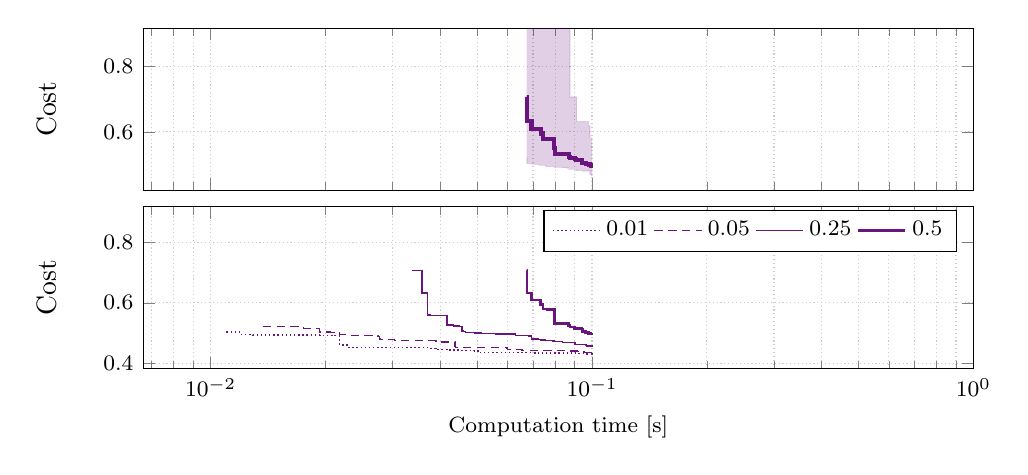
\begin{tikzpicture} [
  xscale=1,
  yscale=1
]
\begin{axis} [
  width=\textwidth,
  height=0.3\textwidth,
  at={(0cm, 0cm)},
  unbounded coords=jump,
  xtick align=inside,
  ytick align=inside,
  axis line style={solid, black},
  name=defaultInformedRRTstarMedianCostAxis,
  xmajorgrids,
  xminorgrids,
  ymajorgrids,
  major grid style={densely dotted, black!20},
  minor grid style={densely dotted, black!20},
  xmin=0.00665588,
  xmax=1,
  ymax=0.917277,
  xmode=log,
  xlabel={{\empty}},
  xlabel style={font=\footnotesize},
  xticklabel={{\empty}},
  xticklabel style={font=\footnotesize},
  ylabel={Cost},
  ylabel style={font=\footnotesize, text depth=0.0em, text height=0.5em},
  ylabel absolute,
  yticklabel style={font=\footnotesize}
]
\addplot [
  line width=0.5,
  color=pdtpurple,
  mark="none",
  const plot,
  name path={defaultInformedRRTstarMedianCostEvolutionUpperConfidence},
  fill opacity=0.2,
  draw opacity=0.1
] table [
  row sep=\\,
  col sep=&
]{
0.0674 & 2.75183\\
0.0874 & 2.75183\\
0.0875 & 0.70681\\
0.0911 & 0.70681\\
0.0912 & 0.632282\\
0.0979 & 0.632282\\
0.098 & 0.618009\\
0.0986 & 0.618009\\
0.0987 & 0.582012\\
0.0999 & 0.582012\\
0.1 & 0.582012\\
};

\addplot [
  line width=0.5,
  color=pdtpurple,
  mark="none",
  const plot,
  name path={defaultInformedRRTstarMedianCostEvolutionLowerConfidence},
  fill opacity=0.2,
  draw opacity=0.1
] table [
  row sep=\\,
  col sep=&
]{
0.0674 & 0.521862\\
0.0675 & 0.503083\\
0.0682 & 0.503083\\
0.0683 & 0.50254\\
0.0693 & 0.50254\\
0.0694 & 0.501393\\
0.0705 & 0.501393\\
0.0706 & 0.500978\\
0.0707 & 0.500392\\
0.0719 & 0.500392\\
0.072 & 0.500104\\
0.0723 & 0.500104\\
0.0724 & 0.499767\\
0.0727 & 0.499767\\
0.0728 & 0.497793\\
0.073 & 0.497793\\
0.0731 & 0.49779\\
0.0751 & 0.49779\\
0.0752 & 0.496947\\
0.0753 & 0.496347\\
0.0756 & 0.496347\\
0.0757 & 0.495435\\
0.0758 & 0.493925\\
0.0792 & 0.493925\\
0.0793 & 0.492915\\
0.0794 & 0.491447\\
0.081 & 0.491447\\
0.0811 & 0.491396\\
0.0831 & 0.491396\\
0.0832 & 0.490227\\
0.0859 & 0.490227\\
0.086 & 0.489312\\
0.0868 & 0.489312\\
0.0869 & 0.48537\\
0.0906 & 0.48537\\
0.0907 & 0.481489\\
0.0943 & 0.481489\\
0.0944 & 0.480687\\
0.0986 & 0.480687\\
0.0987 & 0.469659\\
0.0993 & 0.469659\\
0.0994 & 0.46715\\
0.0997 & 0.46715\\
0.0998 & 0.466826\\
0.0999 & 0.466826\\
0.1 & 0.466826\\
};

\addplot [
  line width=1,
  color=pdtpurple,
  mark=square*,
  mark size=2,
  const plot,
  fill opacity=0.2,
  draw opacity=0
] fill between [
  of =defaultInformedRRTstarMedianCostEvolutionUpperConfidence and defaultInformedRRTstarMedianCostEvolutionLowerConfidence
];
\addplot [
  line width=1.5,
  color=pdtpurple,
  mark="none",
  const plot,
  name path={defaultInformedRRTstarMedianCostEvolution}
] table [
  row sep=\\,
  col sep=&
]{
0.0001 & inf\\
0.0673 & inf\\
0.0674 & 0.70681\\
0.0675 & 0.632282\\
0.0693 & 0.632282\\
0.0694 & 0.609362\\
0.0733 & 0.609362\\
0.0734 & 0.595264\\
0.0743 & 0.595264\\
0.0744 & 0.579349\\
0.0763 & 0.579349\\
0.0764 & 0.576959\\
0.0796 & 0.576959\\
0.0797 & 0.551503\\
0.0798 & 0.551503\\
0.0799 & 0.532992\\
0.0868 & 0.532992\\
0.0869 & 0.525694\\
0.087 & 0.525694\\
0.0871 & 0.524031\\
0.0874 & 0.524031\\
0.0875 & 0.520627\\
0.0899 & 0.520627\\
0.09 & 0.515762\\
0.0905 & 0.515762\\
0.0906 & 0.515218\\
0.0937 & 0.515218\\
0.0938 & 0.513841\\
0.0942 & 0.513841\\
0.0943 & 0.504322\\
0.0962 & 0.504322\\
0.0963 & 0.500973\\
0.0979 & 0.500973\\
0.098 & 0.500019\\
0.0986 & 0.500019\\
0.0987 & 0.49779\\
0.0992 & 0.49779\\
0.0993 & 0.496798\\
0.0999 & 0.496798\\
0.1 & 0.496798\\
};

\end{axis}

\begin{axis} [
  width=\textwidth,
  height=0.3\textwidth,
  at={($(defaultInformedRRTstarMedianCostAxis.south) - (0.0em, 0.6em)$)},
  unbounded coords=jump,
  xtick align=inside,
  ytick align=inside,
  axis line style={solid, black},
  name=defaultInformedRRTstarCostPercentileEvolutionAxis,
  anchor=north,
  xmajorgrids,
  xminorgrids,
  ymajorgrids,
  major grid style={densely dotted, black!20},
  minor grid style={densely dotted, black!20},
  xmin=0.00665588,
  xmax=1,
  ymax=0.917277,
  xmode=log,
  xlabel={Computation time [s]},
  xlabel style={font=\footnotesize},
  xticklabel style={font=\footnotesize},
  ylabel={Cost},
  ylabel style={font=\footnotesize, text depth=0.0em, text height=0.5em},
  ylabel absolute,
  yticklabel style={font=\footnotesize},
  legend style={font=\footnotesize, legend cell align=left, legend columns=-1}
]
\addplot [
  line width=0.5,
  color=pdtpurple,
  mark="none",
  const plot,
  densely dotted,
  name path={defaultInformedRRTstarpercentile0.01CostEvolution}
] table [
  row sep=\\,
  col sep=&
]{
0.0001 & inf\\
0.0109 & inf\\
0.011 & 0.503633\\
0.0118 & 0.503633\\
0.0119 & 0.496347\\
0.0128 & 0.496347\\
0.0129 & 0.493719\\
0.0192 & 0.493719\\
0.0193 & 0.493002\\
0.0211 & 0.493002\\
0.0212 & 0.491447\\
0.0217 & 0.491447\\
0.0218 & 0.460868\\
0.0229 & 0.460868\\
0.023 & 0.452989\\
0.033 & 0.452989\\
0.0331 & 0.45233\\
0.0375 & 0.45233\\
0.0376 & 0.450059\\
0.0389 & 0.450059\\
0.039 & 0.445845\\
0.0416 & 0.445845\\
0.0417 & 0.444428\\
0.0425 & 0.444428\\
0.0426 & 0.444096\\
0.0448 & 0.444096\\
0.0449 & 0.443474\\
0.045 & 0.443081\\
0.0489 & 0.443081\\
0.049 & 0.442004\\
0.0491 & 0.44048\\
0.0502 & 0.44048\\
0.0503 & 0.43713\\
0.0504 & 0.435549\\
0.0707 & 0.435549\\
0.0708 & 0.435039\\
0.0709 & 0.434624\\
0.0904 & 0.434624\\
0.0905 & 0.432386\\
0.0932 & 0.432386\\
0.0933 & 0.432303\\
0.0934 & 0.432205\\
0.0959 & 0.432205\\
0.096 & 0.431963\\
0.0961 & 0.431475\\
0.0962 & 0.431422\\
0.0999 & 0.431422\\
0.1 & 0.431422\\
};
\addlegendentry{0.01}

\addplot [
  line width=0.5,
  color=pdtpurple,
  mark="none",
  const plot,
  densely dashed,
  name path={defaultInformedRRTstarpercentile0.05CostEvolution}
] table [
  row sep=\\,
  col sep=&
]{
0.0001 & inf\\
0.0136 & inf\\
0.0137 & 0.521862\\
0.0174 & 0.521862\\
0.0175 & 0.516163\\
0.0192 & 0.516163\\
0.0193 & 0.503633\\
0.0205 & 0.503633\\
0.0206 & 0.503083\\
0.0211 & 0.503083\\
0.0212 & 0.501277\\
0.0213 & 0.501277\\
0.0214 & 0.500392\\
0.0217 & 0.500392\\
0.0218 & 0.496347\\
0.0227 & 0.496347\\
0.0228 & 0.493719\\
0.0229 & 0.493002\\
0.0246 & 0.493002\\
0.0247 & 0.491447\\
0.0274 & 0.491447\\
0.0275 & 0.491124\\
0.0276 & 0.489312\\
0.0277 & 0.481363\\
0.0278 & 0.478612\\
0.0302 & 0.478612\\
0.0303 & 0.477033\\
0.0304 & 0.475802\\
0.0334 & 0.475802\\
0.0335 & 0.475523\\
0.0355 & 0.475523\\
0.0356 & 0.474954\\
0.0389 & 0.474954\\
0.039 & 0.472001\\
0.0402 & 0.472001\\
0.0403 & 0.471019\\
0.0404 & 0.47082\\
0.0435 & 0.47082\\
0.0436 & 0.47042\\
0.0437 & 0.456631\\
0.0438 & 0.45233\\
0.0598 & 0.45233\\
0.0599 & 0.448477\\
0.06 & 0.44521\\
0.0654 & 0.44521\\
0.0655 & 0.443506\\
0.0715 & 0.443506\\
0.0716 & 0.443081\\
0.0788 & 0.443081\\
0.0789 & 0.441743\\
0.0861 & 0.441743\\
0.0862 & 0.44123\\
0.0863 & 0.440622\\
0.0871 & 0.440622\\
0.0872 & 0.44056\\
0.0916 & 0.44056\\
0.0917 & 0.438553\\
0.0938 & 0.438553\\
0.0939 & 0.437887\\
0.094 & 0.437463\\
0.0953 & 0.437463\\
0.0954 & 0.436553\\
0.0993 & 0.436553\\
0.0994 & 0.436501\\
0.0996 & 0.436501\\
0.0997 & 0.435994\\
0.0998 & 0.434738\\
0.0999 & 0.434738\\
0.1 & 0.434738\\
};
\addlegendentry{0.05}

\addplot [
  line width=0.5,
  color=pdtpurple,
  mark="none",
  const plot,
  name path={defaultInformedRRTstarpercentile0.25CostEvolution}
] table [
  row sep=\\,
  col sep=&
]{
0.0001 & inf\\
0.0337 & inf\\
0.0338 & 0.70681\\
0.0357 & 0.70681\\
0.0358 & 0.632282\\
0.0369 & 0.632282\\
0.037 & 0.560338\\
0.0375 & 0.560338\\
0.0376 & 0.558857\\
0.0389 & 0.558857\\
0.039 & 0.557342\\
0.0415 & 0.557342\\
0.0416 & 0.55676\\
0.0417 & 0.526925\\
0.0433 & 0.526925\\
0.0434 & 0.524031\\
0.0449 & 0.524031\\
0.045 & 0.521862\\
0.0455 & 0.521862\\
0.0456 & 0.506736\\
0.0459 & 0.506736\\
0.046 & 0.50478\\
0.0465 & 0.50478\\
0.0466 & 0.503083\\
0.0473 & 0.503083\\
0.0474 & 0.501393\\
0.049 & 0.501393\\
0.0491 & 0.500392\\
0.051 & 0.500392\\
0.0511 & 0.499767\\
0.0521 & 0.499767\\
0.0522 & 0.49779\\
0.0558 & 0.49779\\
0.0559 & 0.497215\\
0.0596 & 0.497215\\
0.0597 & 0.496947\\
0.0628 & 0.496947\\
0.0629 & 0.496347\\
0.063 & 0.493076\\
0.0639 & 0.493076\\
0.064 & 0.491911\\
0.0668 & 0.491911\\
0.0669 & 0.491447\\
0.0674 & 0.491447\\
0.0675 & 0.491396\\
0.0682 & 0.491396\\
0.0683 & 0.490227\\
0.0693 & 0.490227\\
0.0694 & 0.488294\\
0.0695 & 0.480074\\
0.072 & 0.480074\\
0.0721 & 0.479293\\
0.0724 & 0.479293\\
0.0725 & 0.478174\\
0.0731 & 0.478174\\
0.0732 & 0.477248\\
0.0753 & 0.477248\\
0.0754 & 0.475408\\
0.0766 & 0.475408\\
0.0767 & 0.475385\\
0.0789 & 0.475385\\
0.079 & 0.474542\\
0.0794 & 0.474542\\
0.0795 & 0.473385\\
0.081 & 0.473385\\
0.0811 & 0.472611\\
0.0833 & 0.472611\\
0.0834 & 0.472278\\
0.0836 & 0.472278\\
0.0837 & 0.469659\\
0.0868 & 0.469659\\
0.0869 & 0.468998\\
0.0898 & 0.468998\\
0.0899 & 0.468396\\
0.09 & 0.467598\\
0.0901 & 0.467598\\
0.0902 & 0.465816\\
0.0903 & 0.464452\\
0.0904 & 0.463035\\
0.0906 & 0.463035\\
0.0907 & 0.462192\\
0.0964 & 0.462192\\
0.0965 & 0.4591\\
0.0966 & 0.458005\\
0.0974 & 0.458005\\
0.0975 & 0.4575\\
0.099 & 0.4575\\
0.0991 & 0.457017\\
0.0993 & 0.457017\\
0.0994 & 0.45696\\
0.0999 & 0.45696\\
0.1 & 0.455895\\
};
\addlegendentry{0.25}

\addplot [
  line width=1,
  color=pdtpurple,
  mark="none",
  const plot,
  name path={defaultInformedRRTstarpercentile0.5CostEvolution}
] table [
  row sep=\\,
  col sep=&
]{
0.0001 & inf\\
0.0673 & inf\\
0.0674 & 0.70681\\
0.0675 & 0.632282\\
0.0693 & 0.632282\\
0.0694 & 0.609362\\
0.0733 & 0.609362\\
0.0734 & 0.595264\\
0.0743 & 0.595264\\
0.0744 & 0.579349\\
0.0763 & 0.579349\\
0.0764 & 0.576959\\
0.0796 & 0.576959\\
0.0797 & 0.551503\\
0.0798 & 0.551503\\
0.0799 & 0.532992\\
0.0868 & 0.532992\\
0.0869 & 0.525694\\
0.087 & 0.525694\\
0.0871 & 0.524031\\
0.0874 & 0.524031\\
0.0875 & 0.520627\\
0.0899 & 0.520627\\
0.09 & 0.515762\\
0.0905 & 0.515762\\
0.0906 & 0.515218\\
0.0937 & 0.515218\\
0.0938 & 0.513841\\
0.0942 & 0.513841\\
0.0943 & 0.504322\\
0.0962 & 0.504322\\
0.0963 & 0.500973\\
0.0979 & 0.500973\\
0.098 & 0.500019\\
0.0986 & 0.500019\\
0.0987 & 0.49779\\
0.0992 & 0.49779\\
0.0993 & 0.496798\\
0.0999 & 0.496798\\
0.1 & 0.496798\\
};
\addlegendentry{0.5}

\addplot [
  line width=0.5,
  color=pdtpurple,
  mark="none",
  const plot,
  name path={defaultInformedRRTstarpercentile0.75CostEvolution}
] table [
  row sep=\\,
  col sep=&
]{
0.0001 & inf\\
0.0999 & inf\\
0.1 & inf\\
};
\addlegendentry{0.75}

\addplot [
  line width=0.5,
  color=pdtpurple,
  mark="none",
  const plot,
  densely dashed,
  name path={defaultInformedRRTstarpercentile0.95CostEvolution}
] table [
  row sep=\\,
  col sep=&
]{
0.0001 & inf\\
0.0999 & inf\\
0.1 & inf\\
};
\addlegendentry{0.95}

\addplot [
  line width=0.5,
  color=pdtpurple,
  mark="none",
  const plot,
  densely dotted,
  name path={defaultInformedRRTstarpercentile0.99CostEvolution}
] table [
  row sep=\\,
  col sep=&
]{
0.0001 & inf\\
0.0999 & inf\\
0.1 & inf\\
};
\addlegendentry{0.99}

\end{axis}

\end{tikzpicture}%
\captionof{figure}{\footnotesize \textbf{Top:} Median cost evolution of Informed RRT* with a nonparametric 99\% confidence interval. \textbf{Bottom:} Seven percentiles of the cost evolution of Informed RRT*.}\end{center}

\pagebreak
\begin{appendices}
\section{Configuration}\label{sec:configuration}
\subsection{Experiment}\label{sec:experiment-configuration}
\begin{lstlisting}
{
  "baseDirectory": "/home/ubuntu/Desktop/hzmp_project/pdt/build/benchmarks/",
  "context": "defaultNarrowPassage2D",
  "executable": "benchmark",
  "experimentDirectory": "/home/ubuntu/Desktop/hzmp_project/pdt/build/benchmarks/2025-09-16_12-27-08_defaultNarrowPassage2D",
  "loadDefaultContextConfig": true,
  "loadDefaultObjectiveConfig": true,
  "loadDefaultPlannerConfig": true,
  "loadDefaultReportConfig": true,
  "logFrequency": 10000,
  "maxTime": 0.2,
  "name": "2025-09-16_12-27-08_defaultNarrowPassage2D",
  "numRuns": 100,
  "objective": "defaultPathLength",
  "planners": [
    "defaultInformedHZ",
    "defaultInformedRRTstar"
  ],
  "results": [
    "/home/ubuntu/Desktop/hzmp_project/pdt/build/benchmarks/2025-09-16_12-27-08_defaultNarrowPassage2D/raw/results_0.csv"
  ],
  "seed": 10981397665449740,
  "useOnlyThisConfig": true
}\end{lstlisting}
\subsection{defaultNarrowPassage2D}\label{sec:context-configuration}
\begin{lstlisting}
{
  "boundarySideLengths": [
    1,
    1
  ],
  "collisionCheckResolution": 5e-06,
  "dimensions": 2,
  "goal": [
    0.2,
    0.0
  ],
  "goalType": "GoalState",
  "maxTime": 0.1,
  "objective": "defaultPathLength",
  "passageOffset": 0.1,
  "passageWidth": 0.1,
  "start": [
    -0.2,
    0.0
  ],
  "type": "NarrowPassage",
  "wallOffset": 0.0,
  "wallThickness": 0.2
}\end{lstlisting}
\subsection{Informed HZ}\label{sec:defaultInformedHZ-configuration}
\begin{lstlisting}
{
  "isAnytime": true,
  "options": {
    "goalBias": 0.05,
    "maxEdgeLength": {
      "2d": 0.1,
      "3d": 0.1,
      "4d": 0.1,
      "5d": 0.1,
      "6d": 0.1,
      "7d": 0.1,
      "8d": 0.1
    },
    "numSamplingAttempts": 100,
    "rewireFactor": 1.1,
    "useKNearest": true
  },
  "parameters": {
    "bounds": "-0.5 0.5 -0.5 0.5",
    "goal": "0.2 0.0",
    "obstacles": "-0.5 -0.5,0.5 -0.5,0.5 0.05,-0.5 0.05; -0.5 0.15,0.5 0.15,0.5 0.5,-0.5 0.5",
    "start": "-0.2 0.0"
  },
  "params": {
    "bounds": "-0.5 0.5 -0.5 0.5",
    "goal": "0.2 0.0",
    "obstacles": "-0.5 -0.5,0.5 -0.5,0.5 0.05,-0.5 0.05; -0.5 0.15,0.5 0.15,0.5 0.5,-0.5 0.5",
    "start": "-0.2 0.0"
  },
  "report": {
    "color": "pdtblue",
    "name": "Informed HZ"
  },
  "type": "InformedHZ"
}\end{lstlisting}
\subsection{Informed RRT*}\label{sec:defaultInformedRRTstar-configuration}
\begin{lstlisting}
{
  "isAnytime": true,
  "options": {
    "goalBias": 0.05,
    "maxEdgeLength": {
      "12d": 2.0,
      "14d": 2.4,
      "16d": 3.0,
      "2d": 0.3,
      "32d": 7.0,
      "3d": 0.4,
      "4d": 0.5,
      "6d": 0.9,
      "8d": 1.25
    },
    "numSamplingAttempts": 1,
    "rewireFactor": 1.001,
    "useKNearest": false
  },
  "report": {
    "color": "pdtpurple",
    "name": "Informed RRT*"
  },
  "type": "InformedRRTstar"
}\end{lstlisting}
\end{appendices}
\end{document}
